\pdfoutput=1
\pdfminorversion=5

\begingroup\expandafter\expandafter\expandafter\endgroup
\expandafter\ifx\csname pdfsuppresswarningpagegroup\endcsname\relax
\else
  \pdfsuppresswarningpagegroup=1\relax
\fi

\documentclass[preprint, 11pt]{elsarticle} %  preprint, review, 11pt
%\usepackage[utf8]{inputenc}
%\usepackage{gensymb}
% For Kindle
%\usepackage[a6paper,margin=0.4cm]{geometry} % For Kindle
\usepackage[margin=1in]{geometry}  % For Preprint
\usepackage{setspace}\doublespacing % double line spacing
\usepackage{longtable}
\usepackage{pdflscape}
\usepackage[hyphens]{url}
\biboptions{sort&compress}
\bibpunct{{\unskip~[}}{]}{,}{n}{}{;}

\usepackage[breaklinks=true, linkcolor=blue!20, citecolor=blue!20, colorlinks=true]{hyperref}
\usepackage{graphicx}
\usepackage{caption}
\usepackage{subcaption}
\usepackage{amsmath}
\DeclareMathOperator*{\argmin}{arg\,min}
% Formula subscripts using \ce{}, e.g., \ce{H2SO4}
\usepackage[version=4]{mhchem}
\usepackage{csquotes}
\usepackage{booktabs,multirow}
\usepackage{latexsym,amsmath,amssymb}
\usepackage[section]{placeins} % creates \FloatBarrier  to keep floats in the subsection you want
\usepackage{todonotes}  % use option [disable] to hide them
\usepackage{adjustbox}


\graphicspath{{./figures/}} % put the figures in a 'figures' directory.

%better printing of numbers
\usepackage[T1]{fontenc}
\usepackage[english]{babel}
\usepackage{csquotes}
\usepackage{textcomp}
\usepackage{comment}
\usepackage{soul}

\usepackage[binary-units]{siunitx}
\sisetup{group-separator={,},
     detect-all,
     binary-units,
     list-units = single,
     range-units = single,
     range-phrase = --,
     per-mode = symbol-or-fraction,
     separate-uncertainty = true,
     multi-part-units = single,
     list-final-separator = {, and },
}
\DeclareSIUnit\atm{atm}
\DeclareSIUnit\bar{bar}
\DeclareSIUnit{\calorie}{cal}

\usepackage{array}
\usepackage{ragged2e}
\usepackage[ampersand]{easylist}


\journal{Combustion and Flame}
%FOR ARXIV PURPOSE - REMOVE THE Preprint submitted to... FOOTER
\makeatletter
\def\ps@pprintTitle{%
   \let\@mkboth\@gobbletwo
   \renewcommand{\@oddhead}{}%
   \renewcommand{\@evenhead}{}%
   \renewcommand{\@evenfoot}{}%
   \renewcommand{\@oddfoot}{}%
 }
\makeatother
%%%%





\begin{document}

\begin{frontmatter}

\title{Automatic calculations of reaction kinetics: recent advances and future challenges}

\author[neu]{Nathan~D.~Harms}
\author[neu]{Richard~H.~West}%\corref{cor1}}
%\ead{r.west@northeastern.edu}

\address[neu]{Department of Chemical Engineering\\
Northeastern University, Boston, MA 02115, USA}

%\cortext[cor1]{Corresponding author}


%====================================================================
\begin{abstract}

Detailed reaction mechanisms help us understand and predict complex phenomena in combustion, atmospheric chemistry, and catalytic systems.
These mechanisms often contain hundreds of species and thousands of reactions, for which thermodynamic and kinetic parameters must be specified.
Ideally, parameters come from high fidelity experiments or theoretical calculations, but given the sheer number of parameters, are often estimated.
With the growth of high performance computing, researchers are developing software to automatically perform accurate transition state theory calculations to calculate kinetic parameters. 
This review highlights the recent advances in automated transition state theory calculations, underscores unique features of existing code bases, and proposes future avenues of research.

\end{abstract}


\begin{keyword}
    Chemical kinetic models\sep Model comparison \sep Transition state theory
\end{keyword}

\end{frontmatter}

%%% Comment Definitions
\newcommand{\sks}[2][]
{\todo[caption={#2}, size=\small, color=blue!20,  #1]{\renewcommand{\baselinestretch}{0.5}\selectfont#2\par}}
\sks[inline]{Comments by Krishna}
\newcommand{\rhw}[2][]
{\todo[caption={#2}, size=\small, color=red!20,  #1]{\renewcommand{\baselinestretch}{0.5}\selectfont#2\par}}
\rhw[inline]{Comments by Richard}
\newcommand{\ejm}[2][]
{\todo[caption={#2}, size=\small, color=green!20,  #1]{\renewcommand{\baselinestretch}{0.5}\selectfont#2\par}}
\ejm[inline]{Comments by Emily}
\newcommand{\cx}[2][]
{\todo[caption={#2}, size=\small, color=brown!20,  #1]{\renewcommand{\baselinestretch}{0.5}\selectfont#2\par}}
\cx[inline]{Comments by Chao}
\newcommand{\cjb}[2][]
{\todo[caption={#2}, size=\small, color=gray!20,  #1]{\renewcommand{\baselinestretch}{0.5}\selectfont#2\par}}
\cjb[inline]{Comments by Chris}

\newcommand{\ndh}[2][]
{\todo[caption={#2}, size=\small, color=orange!20,  #1]{\renewcommand{\baselinestretch}{0.5}\selectfont#2\par}}
\ndh[inline]{Comments by Nate}


%%% figure / table functions

\newcommand\figref{Figure~\ref}
\newcommand\tabref{Table~\ref}
\newcommand\eqnref{Equation~\ref}

%\newcommand\figref{Figure~\ref}

%\clearpage

%%%%%%%%%%%%%%%%%%%%%%%%%%%%%%%%%%%%%%%%%%%%%%%%%%%%%%%%%%%%%%%%
\section{Introduction}
% 



Generating detailed microkinetic models is of utmost importance for understanding reaction pathways in combustion \cite{VandeVijver:2015}, atmospheric chemistry \cite{Vereecken:2012}, and catalytic settings \cite{STOLTZE:2000}.
These models often contain hundreds of species and thousands reactions, where each species and reaction require thermodynamic and kinetic parameters, respectively.
Given the size of these models, efforts have been made to generate detailed kinetic models automatically \cite{vandevijver:2015}. 
GRACE \cite{yoneda:1979}, KING \cite{maio:1992}, NetGen \cite{susnow:1997}, EXGAS \cite{warth:2000}, COMGEN \cite{ratkiewicz:2003}, RING \cite{rangarajan:2012}, GENESYS \cite{vandewiele:2012}, and RMG \cite{gao:2016} are a handful of these codes that can generate mechanisms automatically.
Though all of these codes have different ways of generating mechanisms, they all rely on thermochemical and kinetic data to create generate their mechanisms. 
\rhw{Automated mechanism generation. 
- automated
- Several codes (cite them, and a review paper).
- generate models with thousands of reactions
- consider hundreds of thousands or millions (eg. magoon? others?)
- need data.
}
Because this review focuses on the determination of kinetic parameters, discussion of thermochemistry will be omitted.
Kinetic parameters can be obtained from a variety of sources: experiments, estimations, and transition state theory (TST) calculations.
Experimentation is often preferred, but is costly and near impossible for reactions involving multiple radicals or with species that quickly degrade \cite{Sabbe:2005}.
Parameter estimates are often determined by simple rules, generalized across reactions between structurally similar species \cite{Curran:1998bx, cai:2014}. 
Estimations are much faster than both experiments and TST calculations making them advantageous when 
But estimates can be several orders of magnitude incorrect when rules are misapplied or lacking.
TST calculations allow reaction rate constants to be computed from first principles and tend to be accurate within a factor of two \cite{fernandez:2006, Klippenstein:2017eu}, but are computationally expensive and require manual input and trained guesses to find the correct transition state (TS) geometries for just one reaction pathway. 
Given the enormous number of reactions present in detailed reaction mechanisms, TST calculations need to be automated to make use of high-performance computing.
This review identifies tools that perform automated TS searches, describes process workflows, compares key differences, and highlights future goals of automated TST calculations.

%%%%%%%%%%%%%%%%%%%%%%%%%%%%%%%%%%%%%%%%%%%%%%%%%%%%%%%%%%%%%%%%%%%%%%%%%%%%%%%%%%%%
%%%%%%%%%%%%%%%%%%%%%%%%%%%%%%%%%%%%%%%%%%%%%%%%%%%%%%%%%%%%%%%%%%%%%%%%%%%%%%%%%%%%
%%%%%%%%%%%%%%%%%%%%%%%%%%%%%%%%%%%%%%%%%%%%%%%%%%%%%%%%%%%%%%%%%%%%%%%%%%%%%%%%%%%%

\section{Transition State Theory}

%The goal of this section is to describe the basics of TST.

%To understand concepts mentioned further in this review, we suggest reviews on TST \cite{truhlar:1996, Klippenstein:2017eu}, chemical force fields \cite{Harrison:2018, gonzalez:2011}, Hartree-Fock methods \cite{Echenique:2007}, semi-empirical methods \cite{Christensen:2016}, density functional theory (DFT) \cite{Mardirossian:2017mp}, coupled cluster calculations \cite{Sneskov:2012}.

This section serves as a brief overview of TST; we refer the reader to more thorough reviews by Truhlar and coworkers \cite{truhlar:1996} and Klippenstein \cite{Klippenstein:2017eu} for additional information.

TST, also known as activated complex theory, is based on the idea that reactions proceed through an activated complex, or TS.
If the potential energy surface (PES) is followed along the reaction coordinate from reactants to products, the reactants and products are at minima and the TS is at a saddle point, the highest point on the minimum energy pathway (\figref{fig:pes}). 
TST relies on characterizing the reactants, products, and the TS using electronic structure calculations.

The following subsections give a high-level overview of electronic structure calculations: conformational analysis, rotor treatment, and how to use said calculations to calculate kinetic parameters.

\begin{figure}[htbp]
\centering
\begin{subfigure}[t]{.5\textwidth}
  \centering
  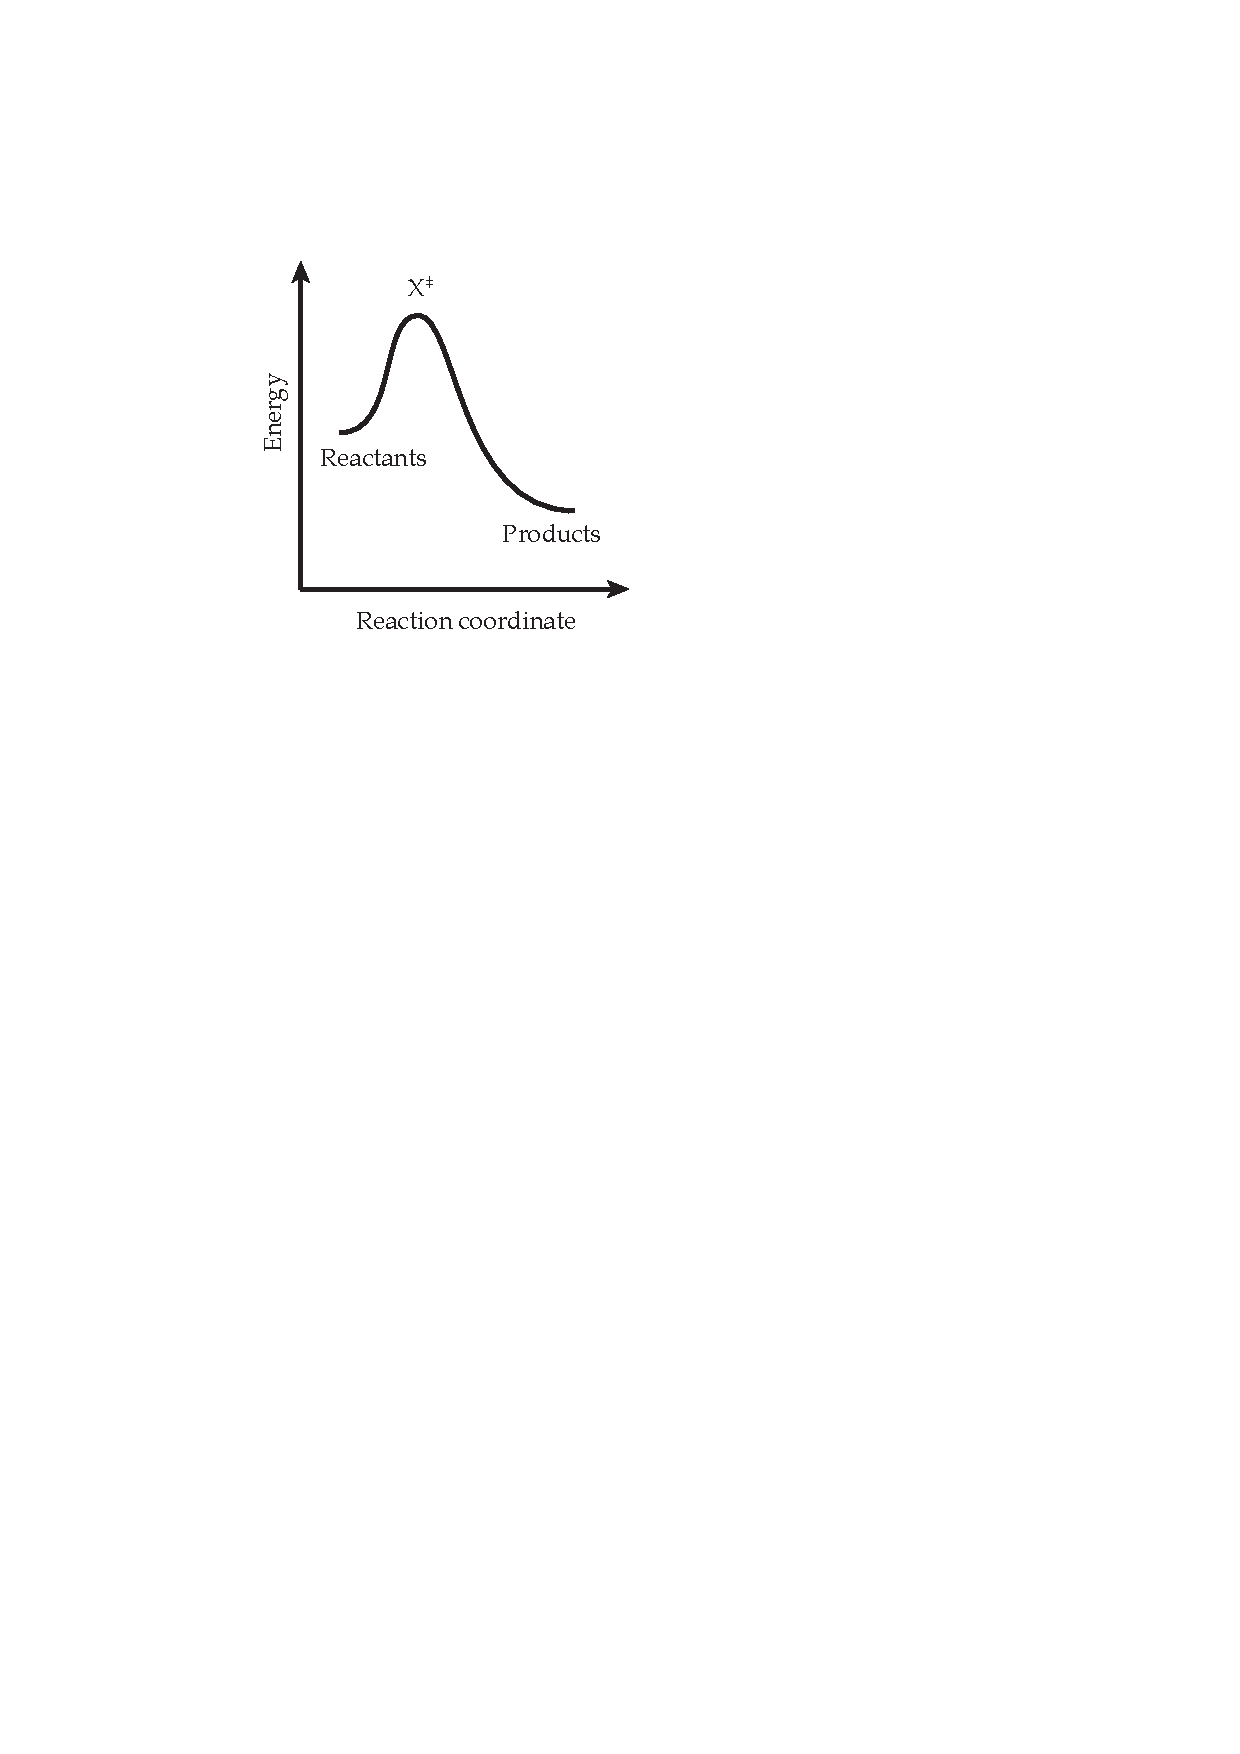
\includegraphics{TST-2D-PES}
  \caption{2-D representation}
  \label{fig:sub1}
\end{subfigure}%
\begin{subfigure}[t]{.5\textwidth}
  \centering
  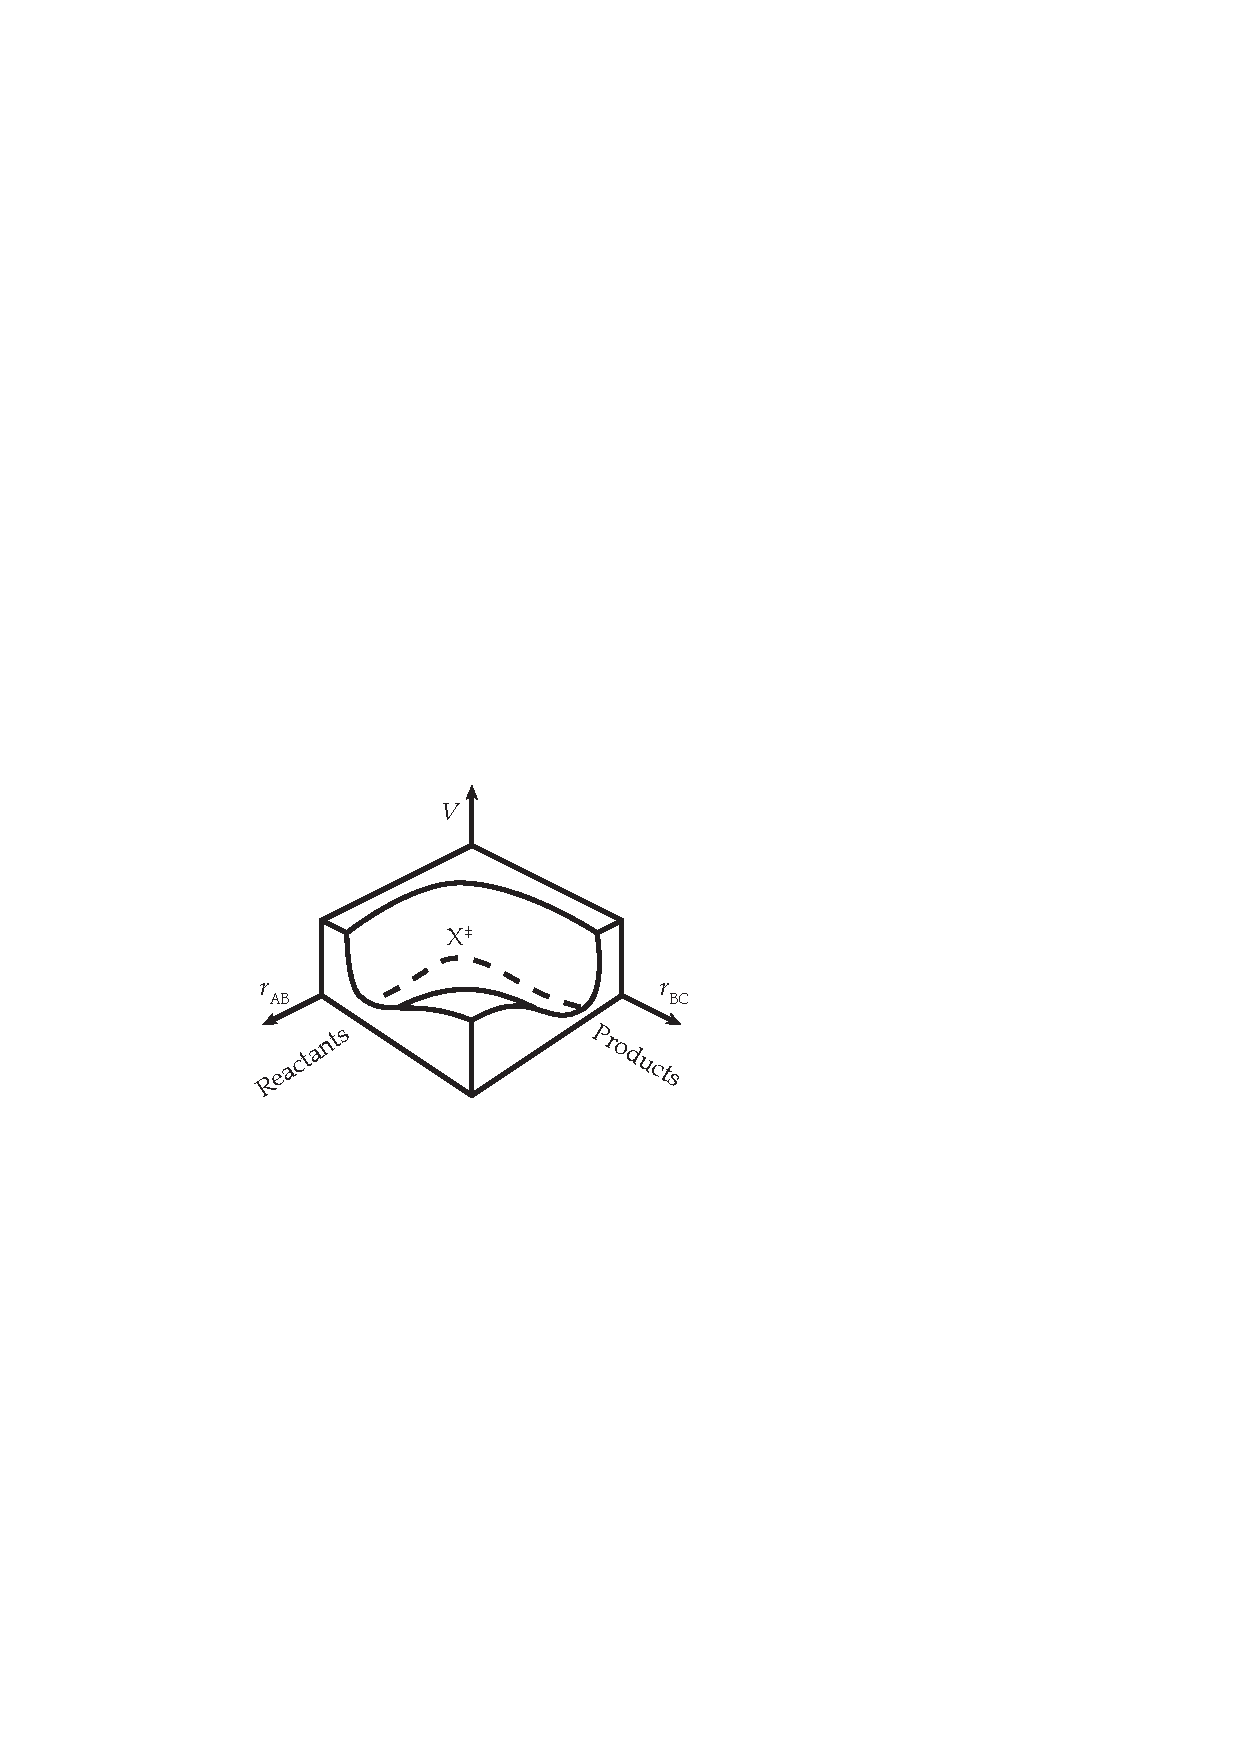
\includegraphics{TST-3D-PES}
  \caption{3-D representation}
  \label{fig:sub2}
\end{subfigure}
\caption{An example potential energy surface for a triatomic reaction \ce{A + BC -> AB + C} . The minima represent the energy of reactant and product geometries while the maximum ($X^\ddagger$) represents the energy of the activated complex, or TS. \rhw[inline]{RHW should upload to figshare and we cite these figures}}
\label{fig:pes}
\end{figure}

\subsection{Electronic structure calculations}


Electronic structure calculations are used to provide energies, forces, and vibrational frequencies when performing geometry optimizations and when characterizing molecules and transition states.
These electronic structure calculations are performed using four broad levels of theory: 
force fields \cite{Harrison:2018, gonzalez:2011}, 
Hartree-Fock (HF)  \cite{Echenique:2007} and semi-empirical calculations \cite{Christensen:2016}, 
density functional theory (DFT) \cite{Mardirossian:2017mp}, 
and coupled cluster calculations \cite{Sneskov:2012},
ranked in \tabref{tab:electronic_structures}.
We suggest the review articles  \citep{Harrison:2018, gonzalez:2011, Echenique:2007, Christensen:2016, Mardirossian:2017mp, Sneskov:2012} to understand how the methods differ.
For the purposes of this article, a higher level of theory will result in higher fidelity calculations and more accurate results,
but will require more computational resources (memory and CPU time).
Additionally, both accuracy and cost of higher level calculations are highly dependent on the choices of quantum method and basis set used; these choices are discussed in depth by Nagy and Jensen \cite{Nagy:2017}.

\begin{table}[htbp]
    \centering
    \begin{tabular}{l | l | l}
        Level of Theory & Theory Description & Examples \\
        \hline
        Level 0 (L0) & Force Fields & UFF \cite{UFF:1992}, MMFF \cite{MMFF94:1996}, AMBER \cite{SalomonFerrer:2012} \\
        Level 1 (L1) & Hartree-Fock and Semi-empirical& HF \cite{HF:1987}, PM3 \cite{PM3:1989} \\
        Level 2 (L2) & Density Functional Theory & M062X \cite{Zhao:2007}, B3LYP \cite{Becke:1993} \\
        Level 3 (L3) & Coupled Cluster & CCSD, CCSD(T) \cite{bartlett:2007}
    \end{tabular}
    \caption{Electronic structure calculation ``Levels of theory''  used in this review with examples.}
    \label{tab:electronic_structures}
\end{table}


%%%%%%%%%%%%
\begin{comment}
\subsubsection{Force fields}

Force fields use attractive and repulsive parameters between atoms to calculate the potential energy of a system \cite{gonzalez:2011}. 
These parameters are often obtained from higher level of theory calculations (e.g. density functional theory or coupled cluster calculations), and describe the forces based on the distance between two bonded atoms, angles between three bonded atoms, torsions between four bonded atoms, non-bonded electrostatic forces, and van der Waals interactions.
Two widely used force fields are the universal force field (UFF) \cite{UFF:1992} and the Merck Molecular force field (MMFF) \cite{MMFF94:1996}.
The UFF uses parameters for bonds, angles, torsions, inversions, electrostatic forces, and van der Waals interactions from literature sources or extrapolations to determine the energy of a complex containing any atom type.
The MMFF includes parameters for the same geometric features as the UFF in addition to parameters for out of plane bending, often resulting in higher fidelity calculations. 
%Parameters for the MMFF are included for all organic atom types and were determined from 2,775 structures optimized with either HF or semi-empirical methods.
Force field calculations are known for giving rough potential energy estimates with little computational resources, and force fields will be referred to as level of theory ``level 0'' (L0).

\subsubsection{Hartree-Fock and semi-empirical methods}

Hartree-Fock methods are a way to approximate the quantum wave function of a molecule at a stationary state \cite{HF:1951, HF:1987} by assuming: the molecular wave function is dependent on the coordinates of each atom's nuclei and their electrons, the solution to the wave function is a linear combination of basis functions, each energy eigenvector is solved by a single Slater determinant, and Coulomb correlations of electrons and London dispersion effects are approximated using mean field theory.
%\todo{HF uses mean field theory to simplify the electron coulomb correlation,  it does not fully neglect it. It is described well on p.34 in Jensen's Introduction to Computational Chemistry book in the DFT QC books folder in Dropbox.  He uses the solar system as an analogy.  In the HF method, you would calculate Earth's orbit by considering the gravitational force from the sun (nucleus) and the average of the gravitational forces from all the other planets}
From these assumptions, Fock matrices are constructed to approximate the energy operator of each orbital of the molecular system using basis functions. \rhw{suggest drop this sentence}

Semi-empirical methods are based on HF methods, but use additional parameters determined from empirical data \cite{SEMethods:2014}. 
By using these empirical data, additional electron correlations and dispersion effects can be accounted for, making these methods slightly more accurate than most HF methods.
HF and semi-empirical methods will be defined as level of theory  ``level 1'' (L1) throughout this paper. 

\subsubsection{Density functional theory}

DFT approximates the wave function using functionals describing the spatial density of electrons in a molecular system, and can be used to approximate the potential acting on electrons \cite{DFT:1964,dft:1994}.
Once the wave function has been approximated, energy and forces can be calculated and minimized to obtain optimized geometries.
Depending on the functionals used, different solutions of the wave function can be approximated, making this method highly dependant on both exchange and correlation interactions. 
In general it is more accurate than HF and semi-empirical methods.
DFT will be defined as a ``level 2'' (L2) level of theory throughout this paper.

\subsubsection{Coupled cluster}

Coupled cluster (CC) methods are another way to describe many-body systems \cite{CC:2002}, and are based on HF molecular orbital methods but instead constructs a mutli-electron wave function to account for electron interactions missing from HF.
These methods offer more accurate treatment of electronic correlation than both HF and DFT, often resulting in high fidelity calculations. 
CC methods are often the most accurate form of calculations that can be performed. However, their increase in accuracy is met by an increase in computational cost.
CC methods include single (S), double (D), triple (T), quadruple (Q) excitations and excitation combinations as well.
One of the more common CC methods is CCSD(T) (the single, double, and pertubative triple excitation) and it was often seen as the ``gold standard'' in that it offers a good balance between accuracy and cost.
The accuracy of CC is highly dependent on the basis set size, and by choosing combinations of different excitation levels, cluster operators are created that can approximate the wave function based on a reference wave function.
Because of the computational cost, these calculations are often reserved for single point (SP) calculations rather than for geometry optimizations.
CC calculations will be defined as a ``level 3'' (L3) level of theory.

%\todo{can have higher order excitations as well (beyond Q),  I would mention CCSD(T) method here which is Single, Double, Pertubative Triple.  It is the most popular methods and known as the 'gold standard' and offers the best accuracy to cost. Going beyond (T) doesn't add much accuracy unless it's a multireference molecule.  You might also want to mention that CC method accuracy is highly dependent on basis set size.  Need to extrapolate to complete basis set limit (CBS) or use F12 with big basis sets}
\end{comment}

\subsection{Conformer Analysis}

Electronic structure calculations are frequently used to optimize geometries to minima or saddle points. 
Depending on the input geometry, the optimization may result an high energy conformation of a molecule when lower energy conformations exist. 
To ensure accuracy of TST calculations, a conformer analysis should be performed to identify many low energy conformations of species and TSs and use these conformers in a Boltzmann distribution to calculate trustworthy thermodynamic and kinetic parameters \cite{Allen:1993, Csaszar:1998}.
This process is trivial for simple geometries, but becomes increasingly complex with the size of the species, many rotatable torsions, rotations about double bonds, and invertible atom centers.

Exploring all of these degrees of freedom will result in a systematic search that is guaranteed to identify the global minima but requires a large amount of computational resources.
Stochastic methods \cite{Ebejer:2012}, such as Monte Carlo or genetic algorithms, involve a guided exploration of a smaller portion of the conformational space to identify low energy conformers, resulting in the lowest energy conformer.
Unfortunately, this is not always the case given the high number of local minima present in species with many conformational degrees of freedom.
\sks[inline]{I think we only search conformational space for equilibrium geometries (0K) but I'm not sure about how you can explain it here. Maybe David has more thoughts on this!}
\subsection{Calculation of Kinetic Parameters}

\subsubsection{Canonical Partition Function}

TST makes a series of assumptions in order to relate the thermodynamic properties of the TS and reactants to the elementary rate of reaction \cite{eyring:1935}. 
First, it is assumed that both reactants and TS are in a quasi-equilibrium state in a vacuum \cite{QSS:2017}.
Additionally, it is assumed that the rate limiting step is the transition from the TS to the products and a modified form of the Eyring equation (\eqnref{eyring:1}) can be written.

\begin{equation}
    k(T) = \kappa(T) \frac{k_B T}{h} \exp{\frac{-\Delta G^\ddagger}{k_B T}}
    \label{eyring:1}
\end{equation}

In \eqnref{eyring:1}, $k_B$ is the Boltzmann constant, $T$ is the temperature, $h$ is Plank's constant, $\Delta G^\ddagger$ is the change in Gibb's energy when progressing from the reactants to the products, $R$ is the ideal gas constant, 
and $\kappa(T)$ is the temperature dependent correction faction for quantum tunneling.
Quantum tunneling is the probability that the reaction will proceed through a barrier that is lower than electronic barrier \cite{RUBAKOV:1984}, thus increasing the apparent rate constant.
The correction factor for quantum tunneling is often derived from either the Eckart model \cite{eckart:1930} or the Wigner model \cite{Winger:1932}.

\begin{comment}

the probability a particle will tunnel through a barrier without having to overcome that barrier \cite{RUBAKOV:1984}.
In the case if tunneling, reactants will form products even if the barrier height is large and system energy is low. 


In the Eckart model, the barrier is based on the following equation:

\begin{equation}
    V(x) = \frac{\hbar^2}{2m}\Big[ \frac{A\exp^x}{1+\exp^x} + \frac{B\exp^x}{(1+\exp^x)^2} \Big]
    \label{eq:v_tunnel}
\end{equation}


In \eqnref{eq:v_tunnel}, $x$ is the reaction coordinate, $V(x)$ is the energy barrier along $x$, and $A$ and $B$ are fitted parameters.
If the constraint $|B| > |A|$ is applied, we are able to determine the reaction coordinate $x_{max}$ where the energy barrier maximum $V(x_{max})$ exists.

\begin{equation}
    x_{max} = \ln \Bigg(\frac{B+A}{B-A} \Bigg)
    \label{eq:xmax}
\end{equation}

\begin{equation}
    V(x_{max}) = \frac{\hbar^2}{2m} \frac{(A+B)^2}{4B}
    \label{eq:vmax}
\end{equation}

Using equations \eqnref{eq:xmax} and \eqnref{eq:vmax} in the one-dimensional Schrodinger equation, the microcanonical tunneling factor $\kappa(E)$ can be solved as the following:

\begin{equation}
    \kappa(E) = 1 - \frac{\cosh(2\pi a - 2\pi b) + \cosh(2\pi d)}{\cosh(2\pi a + 2\pi b) + \cosh(2\pi d)}
    \label{eq:kappae}
\end{equation}

where

\begin{equation}
    2 \pi a = \frac{2\sqrt{\alpha_1 \xi}}{\alpha_1^{-1/2} + \alpha_2^{-1/2}}
\end{equation}

\begin{equation}
    2 \pi b = \frac{2 \sqrt{|(\xi -1)\alpha_1 + \alpha_2| }}{\alpha_1^{-1/2} + \alpha_2^{-1/2}}
\end{equation}

\begin{equation}
    2 \pi d = 2 \sqrt{|\alpha_1 \alpha_2 - 4 \pi^2 / 16|}
\end{equation}

\begin{equation}
    \alpha_1 = 2\pi \frac{\Delta V_1}{h | \nu_{TS}|}
\end{equation}

\begin{equation}
    \alpha_2 = 2\pi \frac{\Delta V_2}{h | \nu_{TS}|}
\end{equation}

\begin{equation}
    \xi = \frac{E}{\Delta V_1}
\end{equation}

In the above equations, $\Delta V_1$ and $\Delta V_2$ is the thermal energy difference between the TS and the reactants and products, respectively, $\nu_{TS}$ is the imaginary frequency of the TS, and $h$ is Planck's constant. 
\eqnref{eq:kappae} can be used to arrive at the canonical tunneling factor as a function of temperature expressed as

\begin{equation}
    \kappa (T) = \exp^{\frac{\Delta V_1}{k_B T}} \int_0^\infty \kappa(E) \exp^{\frac{-E}{k_B T}} dE
\end{equation}

In contrast, the Wigner model \cite{Winger:1932} describes the canonical tunneling factor as follows:

\begin{equation}
    \kappa (T) = 1 + \frac{1}{24} \Big( \frac{h |\nu_{TS}|}{k_B T}\Big)^2
\end{equation}

%The correction factor for tunneling can be calculated through equation \tabref{tunneling}:\rhw{Without specifying $\kappa(E)$ this can't actually be used, so is it helpful for understanding?}
%\begin{equation}
%    \kappa(E) = e^{\frac{V(E)}{kT}} \int^{\infty}_{E_0} \frac{K(E) e^{\frac{-E}{kT}}}{kT} dE
%    \label{tunneling}
%\end{equation}
%where $V$ is the barrier height, $E$ is energy, $E_0$ is the energy of the reactants, and $K(E)$ is the transmission probability for tunneling.\rhw{what's $E_0$} \ndh{answered}

In general, $\kappa(T)$ is dependant on the energy of the system, the shape of the barrier, and the effective mass of the system, described in detail by Brown \cite{Brown:1981}.
\end{comment}

\begin{equation}
    k(T) = \kappa(T) \frac{k_B T}{h} \frac{Q^\ddagger}{\prod^{n}_{i} Q_i} \exp{\frac{-\Delta E^{\ddagger}_{0}}{k_B T}}
    \label{eyring:2}
\end{equation}

\eqnref{eyring:2} can be obtained, from \eqnref{eyring:1}, through statistical thermodynamics and with a tunneling correction, $\kappa(T)$. 
$Q^\ddagger$ represents the canonical partition function of the TS, $\prod^n_i Q_i$ is the product of the partition functions of $n$ number of reactants, $\Delta E^{\ddagger}_0$ is the activation energy for this reaction.
These equations can only be used if the partition functions of the TS, reactants, and products are known. 
The canonical partition function of a species can be represented by the molecular partition function of that species, $q$, and the number of indistinguishable molecules of that species in the system, $N$, as described by \eqnref{eq:q}.

\begin{equation}
    Q = \frac{q^N}{N!}
    \label{eq:q}
\end{equation}


The molecular partition function of a species or a TS can be given by the Boltzmann weighted sum of $i$ energy states given by:
\begin{equation}
    q = \sum_i g_i \exp\left(-\frac{\epsilon_i}{k_B T}\right)
    \label{eq:Q}
\end{equation}
$g_i$ is the degeneracy of the $i$th state, $\epsilon_i$ is the energy level of the $i$th state, $k_B$ is the Boltzmann constant, and $T$ is the temperature of the system.
It can be assumed the energy of each state is the sum of  separable energy contributions across $j$ modes and can be described by \eqnref{eq:epsilon}.

\begin{equation}
    \epsilon_i = \sum_j \epsilon_{j,i}
    \label{eq:epsilon}
\end{equation}

Translational, rotational, vibrational, and electronic contributions to the partition function are commonly used modes.
By combining \eqnref{eq:Q} and \eqnref{eq:epsilon}, we find that the molecular partition function can be represented as the product of molecular partition functions for particular modes (i.e. $q_j$ is the molecular partition function for mode $j$) as shown in \eqnref{qtot}. 
 
\begin{equation}
    q = \prod_j q_j
    \label{qtot}
\end{equation}
%From this point, a set of assumptions can be made in how to arrive at an adequate approximation of the canonical partition function from quantum calculations \cite{Truhlar:1991}.\rhw{what does this sentence add/mean?}


\begin{comment}
The rigid rotor harmonic oscillator approximation is frequently used to calculate the overall partition function.
This approximation treats the bond as a system with a resting equilibrium distance and a force constant that restores changes in bond length to its equilibrium distance.
The total partition function, $Q_{tot}$, is the product of the translational ($Q_{trans}$), rotational ($Q_{rot}$), vibrational ($Q_{vib}$), and electronic ($Q_{elec}$) partition functions of a molecule. 

\begin{equation}
    Q_{tot} = Q_{trans} Q_{rot} Q_{vib} Q_{elec}
    \label{qtot}
\end{equation}

\begin{equation}
    Q_{trans} = V \bigg( \frac{2 \pi M k_B T}{h^2} \bigg)^{\frac{3}{2}}
    \label{qtrans}
\end{equation}

\begin{equation}
    Q_{rot} = \frac{\sqrt{\pi}}{\sigma_{ext}} \bigg( \frac{8 \pi I_m k_B T}{h^2} \bigg)^{\frac{3}{2}} ; I_m = I_x I_y I_z
    \label{qrot}
\end{equation}

\begin{equation}
    Q_{vib} = \prod_i \bigg(1- \exp{\frac{-h \nu_i}{k_B T}} \bigg)^{-1}
    \label{qvib}
\end{equation}

\begin{equation}
    Q_{elec} = \sum_i g_i \exp{\frac{ -\epsilon_{ele,i}}{k_B T}} \approx g_0
    \label{qelec}
\end{equation}

All parameters, aside from constants and temperature, are unique to a specific molecule.
The translational partition function is related to the volume  $V = k_B T/p$, and the  weight of the molecule.
The rotational partition function is related to the moments of inertia, $I_x$, $I_y$ and $I_z$, and the molecular symmetry, $\sigma_{ext}$ -- the determination of which is discussed in subsequent sections.
The vibrational partition function is related to the vibrational frequencies, $\nu_i$, of each vibrational mode in the molecule.
Finally, the electronic partition function is the sum of states over electronic energies, $\epsilon_{ele,i}$, with degeneracies, $g_i$. 
It is often assumed the lowest energy state is the only one available (valid unless the first excited energy level is unusually low) so $Q_{elec}=g_0$.
\end{comment}

\subsubsection{Master equation solvers}

%\ndh{revise this section a lil more in-depth}
% Possibly helpful papers:
% Stephen J. Klippenstein, Carlo Cavallotti. Ab initio kinetics for pyrolysis and combustion systems. 2019,,, 115-167. https://doi.org/10.1016/B978-0-444-64087-1.00002-4
% Nicholas J.B. Green. Steady-state master equation methods. 2019,,, 465-514. https://doi.org/10.1016/B978-0-444-64207-3.00008-1 https://sci-hub.st/10.1016/B978-0-444-64207-3.00008-1
% Stephen J. Klippenstein. From theoretical reaction dynamics to chemical modeling of combustion. Proceedings of the Combustion Institute 2017, 36 (1) , 77-111. https://doi.org/10.1016/j.proci.2016.07.100
% Stephen J. Klippenstein, Vijay S. Pande, and Donald G. Truhlar . Chemical Kinetics and Mechanisms of Complex Systems: A Perspective on Recent Theoretical Advances. Journal of the American Chemical Society 2014, 136 (2) , 528-546. https://doi.org/10.1021/ja408723a
% Yuri Georgievskii, James A. Miller, Michael P. Burke, and Stephen J. Klippenstein . Reformulation and Solution of the Master Equation for Multiple-Well Chemical Reactions. The Journal of Physical Chemistry A 2013, 117 (46) , 12146-12154. https://doi.org/10.1021/jp4060704
% Joshua W. Allen, C. Franklin Goldsmith, William H. Green. Automatic estimation of pressure-dependent rate coefficients. Phys. Chem. Chem. Phys. 2012, 14 (3) , 1131-1155. https://doi.org/10.1039/C1CP22765C
% Antonio Fernández-Ramos, , James A. Miller and, Stephen J. Klippenstein, , Donald G. Truhlar. Modeling the Kinetics of Bimolecular Reactions. Chemical Reviews 2006, 106 (11) , 4518-4584. https://doi.org/10.1021/cr050205w
%James A. Miller, , Stephen J. Klippenstein. Master Equation Methods in Gas Phase Chemical Kinetics. The Journal of Physical Chemistry A 2006, 110 (36) , 10528-10544. https://doi.org/10.1021/jp062693x
% Terry J. Frankcombe, Sean C. Smith. Selecting Methods to Solve Multi-Well Master Equations. Journal of Theoretical and Computational Chemistry 2003, 02 (02) , 179-191. https://doi.org/10.1142/S0219633603000483

This review focuses on automating the application of Ab Initio Transition State Theory.
For reactions involving recombination, dissociation, unimolecular isomerization, or multiple wells,  non-reactive collisional energy transfer can play a crucial role and   a Master Equation (ME) treatment is required \cite{Pilling:2003, truhlar:1996, 10.1126/science.aaa1257,10.1126/science.1260856}\rhw{check these are best references}. The master equation represents the time-varying energy-resolved populations of the isomers, considering collisional energy transfer as well as microcanonical reaction rates.\cite{Klippenstein:2017eu}.
Master equation solvers can be used to calculate phenomenological kinetic parameters for reactions involving multiple wells and pressure dependence, including van der Walls complexes.
Master equation solvers include Arkane (formally CanTherm) \cite{gao:2016}, MultiWell
\cite{?,?}\rhw{Barker, J. R. Multiple-Well, Mulitple-Path Unimolecular Reaction Systems. I. MultiWell Computer Program Suite. Int. J. Chem. Kinet. 2001, 33, 232-245.}
\rhw{Barker, J. R.; Nguyen, T. L.; Stanton, J. F.; Aieta, C.; Ceotto, M.; Gabas, F.; Kumar, T. J. D.; Li, C. G. L.; Lohr, L. L.; Maranzana, A.; Ortiz, N. F.; Preses, J. M.; Sonk, J. A.; Stimac, P. J. Mutiwell-2017 Software Suite; Barker, J. R. University of Michigan, Ann Arbor, Michigan, USA. http://clasp-research.engin.umich.edu/multiwell/ }
,  MESS \cite{MESS:2013}, and MESMER \cite{MESMER:2012}.
%MESS and MESMER follow the complete master equation methodology \cite{truhlar:1996} while Arkane follow the Rice--Ramsperger--Kassel--Marcus (RRKM) approximation \cite{RRKM:1999}. 

A Master Equation approach still requires microcanonical reaction rates and hence characterization of the reactants, products, and transition states, so the results from any of the automated TS-locating tools can be used for performing ME calculations. However, of the tools reviewed, only EStokTP (via MESS), KinBot (via MESS or MESMER), and to some extent AutoTST (via RMG and Arkane) attempt to automate the ME calculations themselves.




\subsubsection{Internal rotors}

An internal rotor is a non-terminal bond with rotatable groups of atoms, or tops, on either end (e.g. the C-C bond in ethane). 
An internal rotor can be treated as a free rotor, a rigid rotor, or a hindered rotor.
A free rotor is assumed to have no rotational barrier; an appropriate assumption at low barrier to temperatures ratios (V/T), but incorrect for high ratios.
In the rigid rotor approximation, the calculated frequencies are treated as harmonic oscillators with the optimized geometry as the equilibrium point and the corresponding displacements about this geometry are modeled as harmonic motion within an inescapable potential energy well.
At high ratios, the harmonic oscillator approximation holds true. 
Hindered rotors occur at intermediate ratios where the compound has enough energy to rotate out of one conformer and into another, but not enough energy for hindrance to be negligible.

The calculation of the partition function can be further expanded by using the 1-D hindered rotor approximation \cite{pitzer:1942, pfaendtner:2007, Lin:2008}. 
In this approximation, each side of a four atom dihedral is considered a separable rotatable top.
Starting from a minimum energy structure, the potential energy is determined using electronic structure calculations as one top is rotated over \ang{360} for asymmetric tops or over $\ang{360}/\sigma$ for symmetric tops where $\sigma$ is the degree of rotational symmetry of that top. 
It is noted that the description represents separable 1-D hindered rotors.

Coupled hindered rotors (e.g. 2-D and 3-D) involve a grid like search where rotations about multiple tops are investigated at the same time. 
These calculations can result in even more accurate treatment of hindered rotation in a species but require much more computation time.
More in depth discussion of coupled hindered rotors is discussed in reference \cite{fernandez:2013}.


\subsubsection{Symmetry number}

A symmetry number is the number of equivalent orientation of a molecule that can be found as a result of rotation \cite{Lynch:2004, gilson:2010}.
This can be broken down further into internal symmetry ($sigma_{int}$, symmetry by modification of internal coordinates) and external symmetry ($\sigma_{ext}$, symmetry by rotations of the entire fixed molecule).
The total symmetry is simply the product of the internal and external symmetry.
Determining the external symmetry number of species and TS geometries is imperative because it is included in the rotational partition function ($q_{rot}$) as shown in \eqnref{eq:q_rot}.

\begin{equation}
    q_{rot} = \frac{\pi^{1/2}}{\sigma_{ext}}\Big(\frac{8 \pi^2 I_A k_B T}{h^2}\Big)^{1/2} \Big(\frac{8 \pi^2 I_B k_B T}{h^2}\Big)^{1/2} \Big(\frac{8 \pi^2 I_C k_B T}{h^2}\Big)^{1/2}
    \label{eq:q_rot}
\end{equation}

In the above equation, $\sigma_{ext}$ is the external symmetry, $I_A$, $I_B$, and $I_C$ are the principal moments of inertia, $k_B$ is the Boltzmann constant, $T$ is the temperature, and $h$ is Plank's constant. 
\eqnref{eq:q_rot} represents the rotational contributions to the molecular partition function and is included in \eqnref{qtot} and subsequently in the rate expression, \eqnref{eyring:2}. 
We suggest readers review Refs. \cite{FernandezRamos:2007, Pollak:1978} for a detailed description of symmetry numbers in chemical kinetics.


\begin{comment}
For a majority of cases, rotational symmetry numbers are adequate when describing the overall external symmetry number of stable species and can be calculated using \eqnref{eq:symm}.

\begin{equation}
    \label{eq:symm}
    \sigma_{ext} \approx \sigma_{rot} = \frac{m!}{n_d}
\end{equation}

In the above equation, $\sigma$ is the rotational symmetry number, $m!$ is the number of permutation of $m$ equivalent atoms, and $n_d$ is the number of distinguishable configurations or orientations of molecules that cannot be mapped onto another configuration by rotation.
For example, when considering ammonia (\ce{NH3}), there are three equivalent hydrogen atoms and two distinguishable configurations of those atoms resulting in a rotational symmetry number of three.
Rotational symmetry numbers of TS geometries can be taken as the product of the rotational symmetry numbers of the stable species, shown in equation \eqnref{eq:symm_ts}, where $n$ is the number of reactants in a reaction and $\sigma_{rot,i}$ is the rotational symmetry number for the $i$th reactant.

\begin{equation}
    \sigma_{TS,rot} = \prod^n_{i=1}\sigma_{rot,i}
    \label{eq:symm_ts}
\end{equation}

For TSs of bimolecular reactions between identical species, the rotational symmetry number is not sufficient when determining the overall symmetry number of a geometry.
In this case, it is better to use the rotational translational symmetry number, $\sigma_{r-t}$, which takes into account translational symmetry.
For example, assume the reaction \ce{A_i + A_j -> Products} has a TS geometry, $R$, where $i$ and $j$ are labels to distinguish between identical \ce{A} species.
In this case, the rotational symmetry number would be $\sigma_{rot,R} = \sigma_{rot,A}^2$ but this does not account for the translation of identical molecule (e.g. \ce{A_i + A_j} in 3D space compared to \ce{A_j + A_i}), so the rotational translational symmetry number would be $\sigma_{rot,R} = 2\sigma_{rot,A}^2$. 
The factor of two accounts for the translational exchange of positions of \ce{A_i} and \ce{A_j} via translation.
Additional explanations of symmetry numbers are described by Fern\'andez-Ramos and co-workers \cite{FernandezRamos:2007}.
\end{comment}

%%%%%%%%%%%%%%%%%%%%%%%%%%%%%%%%%%%%%%%%%%%%%%%%%%%%%%%%%%%%%%%%%%%%%%%%%%%%%%%%%%%%
%%%%%%%%%%%%%%%%%%%%%%%%%%%%%%%%%%%%%%%%%%%%%%%%%%%%%%%%%%%%%%%%%%%%%%%%%%%%%%%%%%%%
%%%%%%%%%%%%%%%%%%%%%%%%%%%%%%%%%%%%%%%%%%%%%%%%%%%%%%%%%%%%%%%%%%%%%%%%%%%%%%%%%%%%


\section{Automated transition state theory code bases}

This section of the review introduces existing code bases capable of performing automated TST calculations, highlights and compares each code's key features and methodologies, and discusses test sets.
The software reviewed are as follows:
\begin{itemize}
    \item Freezing String Methods \cite{Behn:2011}
    \item molecularGSM \cite{Peters:2004,Zimmerman:2013jctc,Zimmerman:2013jcp,Zimmerman:2015jcc}
    \item AutoMeKin \cite{Martinez:2015,Martinez:2015jccp,rodriguez:2018,mopac:2016}
    \item AutoTST \cite{Bhoorasingh:2015,bhoorasingh:2017}
    \item AFIR \cite{Maeda:2016, Madea:2018}
    \item AutoTS \cite{jacobson:2017}
    \item Genesys \cite{VANDEVIJVER:2018, vandewiele:2012}
    \item AAROM \cite{Guan:2018}
    \item EStokTP \cite{Cavallotti:2019jctc}
    \item KinBot \cite{kinbot:2018, kinbot:2019}
    \item TS Gen \cite{grambow:2020, pattanaik:2020}
    \item RMSD-PP-TS \cite{rasmussen:2020}
    \item autodE \cite{young:2020}
\end{itemize}

%%%%%%%%%%%%%%%%%%%%%%%%%%%%%%%%%%%%%%%%%%%%%%%%%%%%%%%%%%%%%%%%%%%%%%%%%%%%%%%%%%%%
%%%%%%%%%%%%%%%%%%%%%%%%%%%%%%%%%%%%%%%%%%%%%%%%%%%%%%%%%%%%%%%%%%%%%%%%%%%%%%%%%%%%
%%%%%%%%%%%%%%%%%%                                                %%%%%%%%%%%%%%%%%%
%%%%%%%%%%%%%%%%%%                     String Methods                    %%%%%%%%%%%%%%%%%%
%%%%%%%%%%%%%%%%%%                                                %%%%%%%%%%%%%%%%%%
%%%%%%%%%%%%%%%%%%%%%%%%%%%%%%%%%%%%%%%%%%%%%%%%%%%%%%%%%%%%%%%%%%%%%%%%%%%%%%%%%%%%
%%%%%%%%%%%%%%%%%%%%%%%%%%%%%%%%%%%%%%%%%%%%%%%%%%%%%%%%%%%%%%%%%%%%%%%%%%%%%%%%%%%%

\subsection{Freezing String Methods (2011)}

The freezing string method (FSM) is an iterative TS search method that uses both reactant and product geometries in an iterative double ended search \cite{Behn:2011}.
First, an interpolated path between user provided reactant and product complexes along a PES is drawn.
FSM will step reactant and product geometries along this path by a user specified inward step size and partially optimize complexes perpendicularly to the path. 
The resultant complexes are then used to draw a new interpolation and this process is iterated.
The optimization of these new complexes is performed using a conjugated gradient scheme for a specific number of steps of limited size. 
%The optimization is constrained such that no step will change the Cartesian position of any atom by greater than 0.05 \si{\angstrom} and is stopped if the distance between optimizing complexes exceeds a distance that is greater than initial distance between the new nodes plus one half of the step size. \rhw{too much detail?}
This process is repeated until the entire string connecting the two initial complexes is known. 
A representation of this process is shown in \figref{fig:fsm}. 

\begin{figure}[htbp]
    \centering
    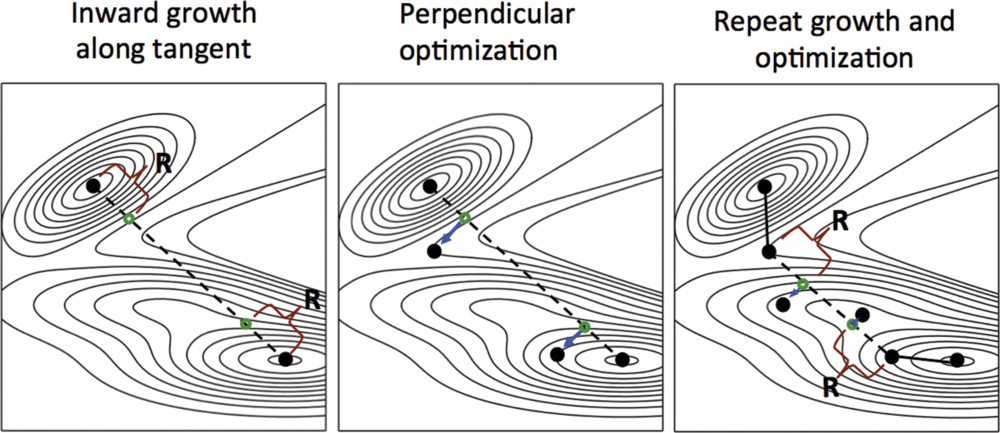
\includegraphics[width=5in]{fsm}
    \caption{Cartoon representation of the freezing string method over an example PES. From \cite{Behn:2011}}
    \label{fig:fsm}
\end{figure}
%\rhw{do you have permission from publishers yet? often just a form to complete on their website}

Interpolations between complexes is performed either using Cartesian interpolation or linear synchronous transit (LST) interpolation \cite{HALGREN:1977, Peng:1993}. 

One or more complexes, or nodes, along the string are used to perform exact TS searches.
Often the highest energy complex is used, however, more can be used for a complete search of more complex reactions. 
Successfully optimized (i.e. converged) TSs are validated through intrinsic reaction coordinate (IRC) calculations \cite{Maeda:2015} which verifies that the TS corresponds to the correct input reactant and product geometries. 

All levels of theory available in Q-Chem \cite{QChem:2015}, an electronic structure calculator, can be used when using FSM, although the authors used L2 level of theory calculations for three reactions in their preliminary study: the conversion of cis,cis-2,4-hexadiene to trans-3,4-dimethylcyclobutene; the alanine dipeptide $C5$ to $C_{7AX}$ isomerization; and metallacycle formation in a Ni-exchanged zeolite \cite{Behn:2011}. %The FSM workflow was also compared against the growing string method, another code base described later.
Another research goal was to compare efficacy and computational time between the FSM workflow and the growing string method described in the following section.

\subsection{molecularGSM (2011)}

The growing string method (GSM) was developed by Peters and co-workers \cite{Peters:2004} and maintained by Paul Zimmerman and his research group in molecularGSM \cite{Zimmerman:2013jctc,Zimmerman:2013jcp, Zimmerman:2015jcc} and is described in \figref{fig:gsm}.
The molecularGSM is similar to the FSM; both involve a double ended ``string'' that connects the reactant and product wells which incrementally step along a reaction path.
However, the difference between FSM and molecularGSM is how such steps are taken. 

Starting from user provided reactant and product wells, molecularGSM draws an interpolation between these nodes and new nodes are created one step inwards along that path. 
Nodes on the string are optimized until the gradient on the PES is below an optimization threshold and a new interpolation is made using \textit{all} nodes along the string in contrast to the FSM which only uses the two most center nodes when creating its next interpolation.
This process is repeated, adding additional nodes until the string is optimized and a new interpolation is made between all nodes to find an energy maximum. 
The energy maximum is used to perform a direct TS search.
%Interpolation methods differ between variations of GSM methods used which can be as simple as spline fits to more robust path curvature evaluations \todo{cite different ways which the path can be fitted}.

In addition to a double ended method, molecularGSM has a single ended method, as described in \figref{fig:se-gsm}.
This process works similarly to the double ended method, but only half of the string is used to find a TS.
This process will iteratively grow the string by adding frontier nodes to the reactant side of the string. 
The path will be interpolated in a similar fashion to the double ended molecularGSM.
When a new frontier node is added and optimized, the frontier node is checked to see if (1) the frontier node is a lower energy than the previous node and (2) the frontier node's constraint gradient on the PES is positive. 
If these two checks pass, all nodes along the string are optimized and the highest energy node is used for a direct TS search.
The final node in the single ended method is then optimized to product geometries.


\begin{figure}[htbp]
    \centering
    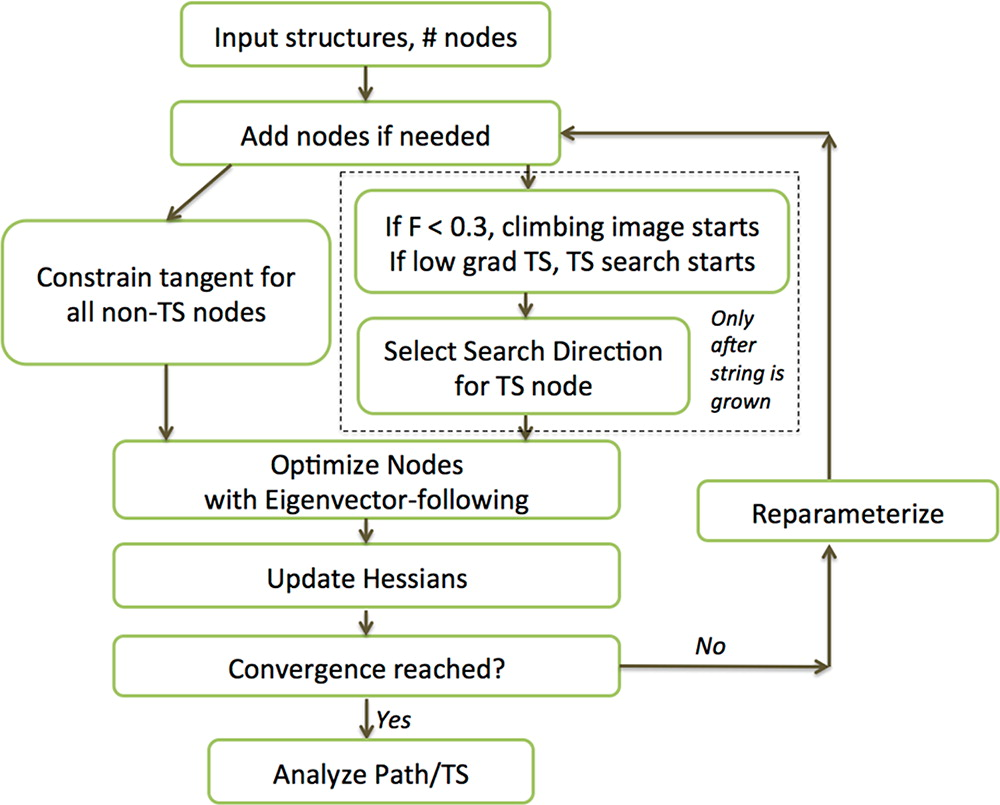
\includegraphics[width=5in]{gsm}
    \caption{Workflow for the double ended growing string method utilized in molecularGSM. Borrowed from \cite{Zimmerman:2013jctc}.}
    \label{fig:gsm}
\end{figure}

\begin{figure}[htbp]
    \centering
    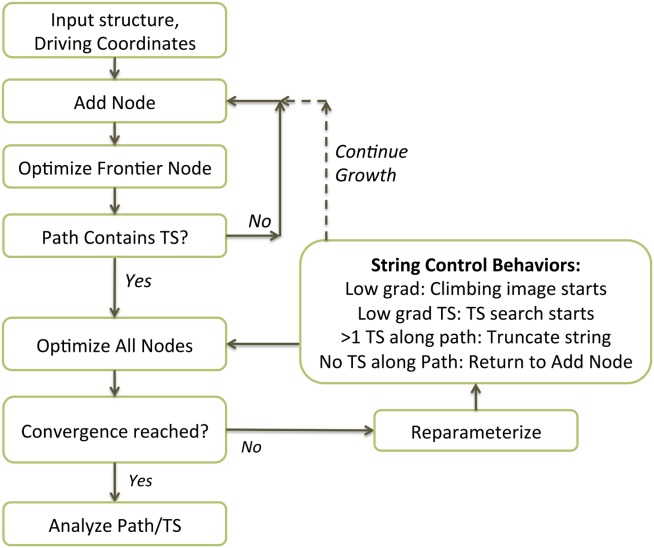
\includegraphics[width=5in]{se-gsm}
    \caption{Workflow for the single ended growing string method utilized in molecularGSM. Borrowed from \cite{Zimmerman:2015jcc}.}
    \label{fig:se-gsm}
\end{figure}

molecularGSM has been tested over a diverse set of uni- and bimolecular reactions including H, N, C, O, Si, Cl, F, P, and B atoms.
Reported success rates are between 58--100\%, depending on user specified variables such as number of nodes along the string or optimization thresholds \cite{Zimmerman:2013jctc, Zimmerman:2013jcp, Zimmerman:2015jcc, Jafari:2017, Roessler:2018, Aldaz:2018}.


%%%%%%%%%%%%%%%%%%%%%%%%%%%%%%%%%%%%%%%%%%%%%%%%%%%%%%%%%%%%%%%%%%%%%%%%%%%%%%%%%%%%
%%%%%%%%%%%%%%%%%%%%%%%%%%%%%%%%%%%%%%%%%%%%%%%%%%%%%%%%%%%%%%%%%%%%%%%%%%%%%%%%%%%%
%%%%%%%%%%%%%%%%%%                                                %%%%%%%%%%%%%%%%%%
%%%%%%%%%%%%%%%%%%                     AutoMeKin                  %%%%%%%%%%%%%%%%%%
%%%%%%%%%%%%%%%%%%                                                %%%%%%%%%%%%%%%%%%
%%%%%%%%%%%%%%%%%%%%%%%%%%%%%%%%%%%%%%%%%%%%%%%%%%%%%%%%%%%%%%%%%%%%%%%%%%%%%%%%%%%%
%%%%%%%%%%%%%%%%%%%%%%%%%%%%%%%%%%%%%%%%%%%%%%%%%%%%%%%%%%%%%%%%%%%%%%%%%%%%%%%%%%%%

\subsection{AutoMeKin (2014)}

Initially developed by Mart\'{i}nez-N\'{u}\~{n}ez, AutoMeKin, formerly TSSCDS, performs TS searches using a chemical dynamics simulations methodology \cite{Martinez:2015,Martinez:2015jccp,rodriguez:2018,mopac:2016}.
The general AutoMeKin workflow, as described in \figref{fig:tsscds}, starts by optimizing an input geometry to an energy minimum and calculates vibrational frequencies using a L1 level of theory.
These vibrational modes are used as trajectories for multiple parallel chemical dynamics simulations (CDS) that run over a 20 fs time length.
At each time step for each trajectory, AutoMeKin employs a Bond Breakage / Formation Search (BBFS) algorithm \cite{Kopec:2019} to identify bond are breakage and formation.
%BBFS creates a connectivity matrix that describes pairwise adjacency between atoms. 
%Elements in the matrix are either one for neighboring atoms or zero for non neighboring atoms.\rhw{I think this whole section is too much detail. There's an algorithm to detect when bonds have changed, indicating a reaction}
%Atoms are defined as neighboring if the distance between atoms is less than 10\% of the sum of the covalent radii of the atoms. 
A TS is assumed to exist for a CDS if any bond changes occur and the geometry at which this change occurs is taken as the starting guess for the TS.

All starting guesses are optimized to a saddle points at a low L1 level of theory and resulting TSs are screened to detect and discard duplicates.
The remaining unique TSs undergo IRC calculations to find stable minima on either side of the saddle point, which are subsequently optimized at a higher L2 level of theory. 
TSs are then optimized with a higher L2 level of theory and IRC calculations are performed again to ensure the reaction path is maintained.

\begin{figure}[htbp]
    \centering
    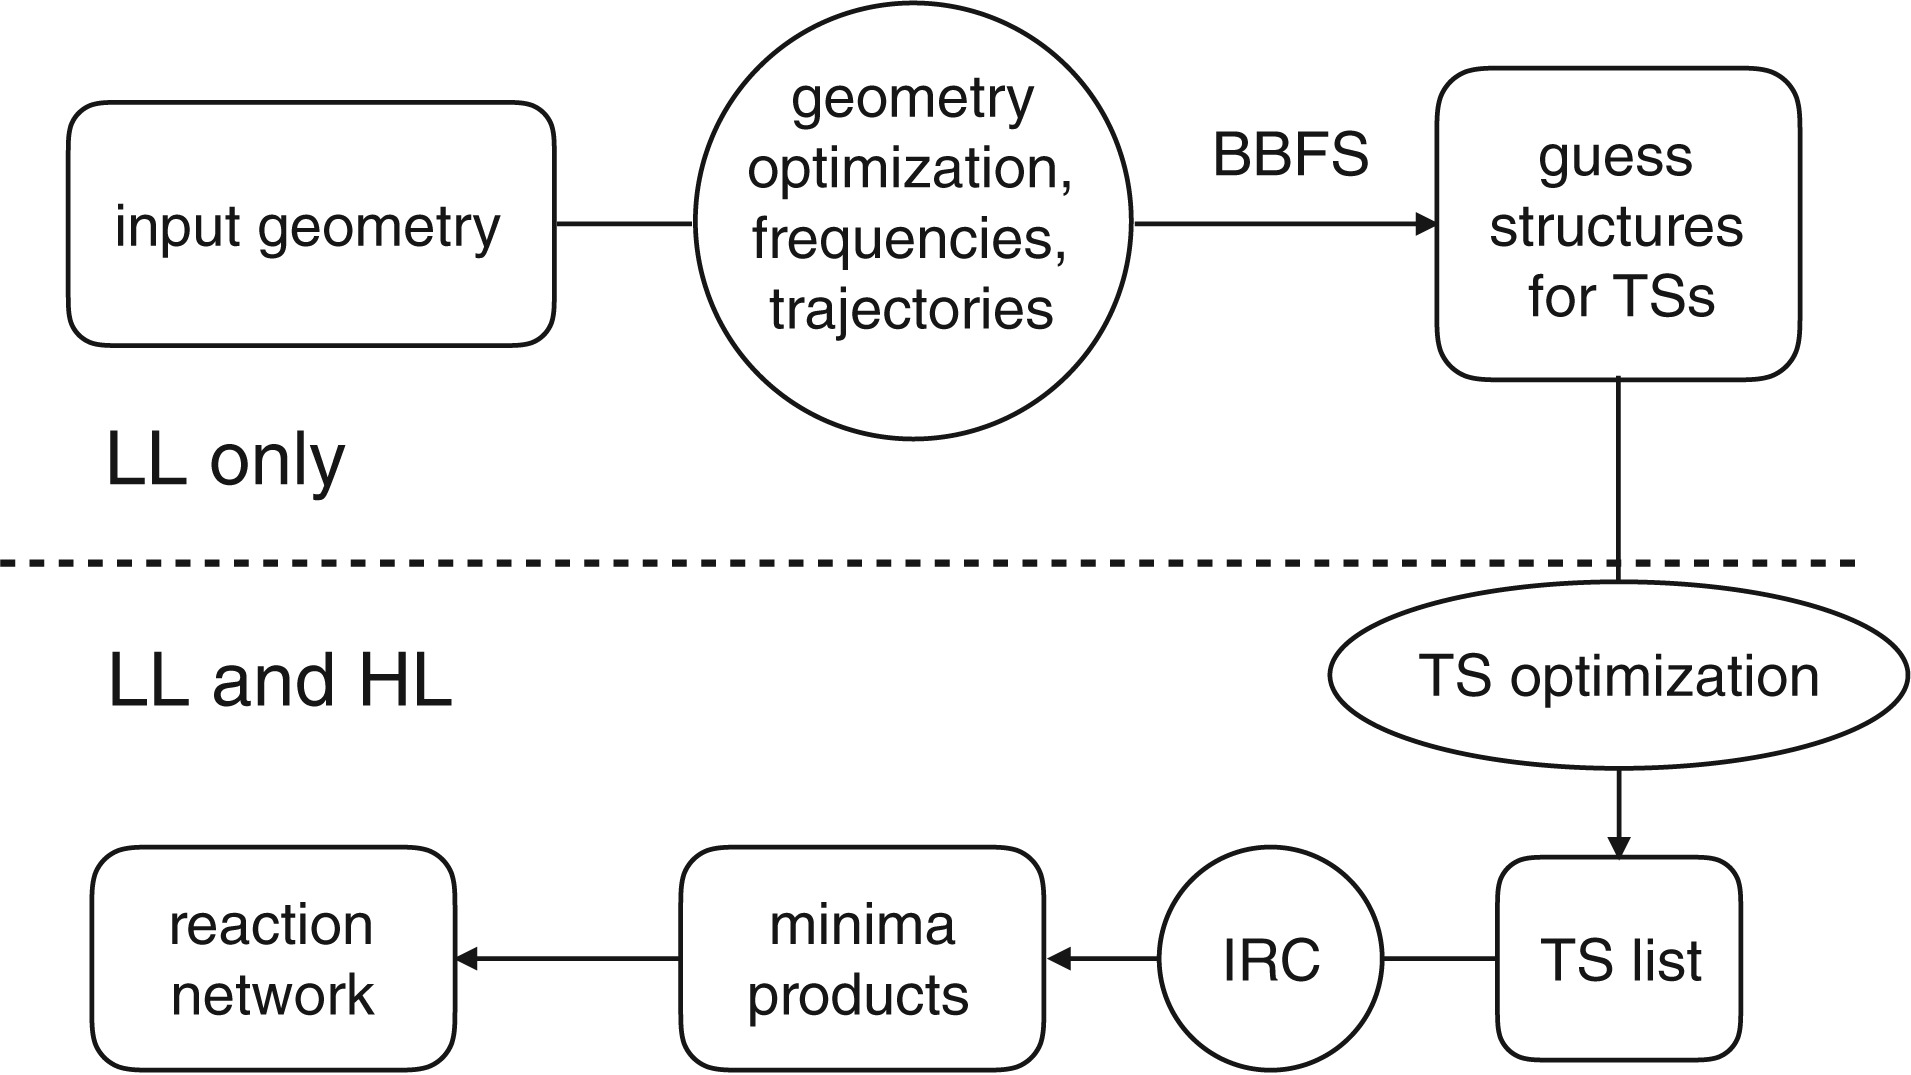
\includegraphics[width=5in]{tsscds}
    \caption{A flow chart describing AutoMeKin. LL stands for the L1 level of theory (low level) and HL is the L2 level of theory (high level). Taken from \cite{Kopec:2019}}
    \label{fig:tsscds}
\end{figure}



\begin{comment}
The AutoMeKin workflow was not designed to consider non-covalent bonds because the distance between non-covalently bond atoms is often too large for the cutoff described above \cite{Kopec:2019}.
Because of this, TSSCDS was modified to work with systems including non-covalent bonds such as vdW complexes, hydrogen bonds, and Lewis acids and bases.

\rhw{this section seems weirdly in depth}
vdW treatment in AutoMeKin starts with a user specified geometry containing the number of reacting fragments and the number of atoms.
From this input, a connectivity matrix, $\textbf{\textit{C}}$, is construction to describe the intra- and intermolecular distances of pairwise atoms.
Consider a system with two molecules, fragments $\textit{A}$ and $\textit{B}$, the connectivity matrix $\textbf{\textit{C}}$ would be depicted by equation \eqnref{eq:C} where $\textbf{\textit{A}}$ and $\textbf{\textit{B}}$ represent the intramolecular distances of fragments $\textit{A}$ and $\textit{B}$, respectively, while $\textit{\textbf{AB}}$ represents the intermolecualar distances.
Elements in matrix $\textbf{\textit{C}}$ are either one or zero to denote if pairwise atoms are bound to each other.
For the diagonal matrices $\textbf{\textit{A}}$ and $\textbf{\textit{B}}$, elements are assigned a one if the distance between atoms are less than 10\% greater than the sum of covalent radii else values are zero.
For matrix $\textbf{\textit{AB}}$, elements are assigned a one if the distance between atoms are less than 10\% greater than the sum of van der Waals radii of the two atoms.

\begin{equation}
    \textbf{\textit{C}} = \begin{pmatrix}
\textbf{\textit{A}} & \textbf{\textit{AB}} \\
\textbf{\textit{AB}} & \textbf{\textit{B}}
\end{pmatrix}
\label{eq:C}
\end{equation}

The remainder of the van der Walls  treatment in AutoMeKin method mirrors the original AutoMeKin method with a few caveats.
Users can specify if fragments are flexible or rigid.
Rigid fragments are ones where intramolecular parameters are frozen while intermolecular parameters are not and flexible fragments are ones where both inter- and intramolecular parameters are not fixed. 
Setting fragments as flexible or rigid can help identify an upper bound of the interaction energy between the two fragments but the flexible setting can offer a complete description of the interactions.
\end{comment}

AutoMeKin is a mature code and has been tested on a variety of systems such as both uni- and bimolecular reactions \cite{Martinez:2015,Martinez:2015jccp,rodriguez:2018,Kopec:2019}.
Although users are able to provide only a single input geometry, the developers of AutoMeKin recommend starting from several initial structures to search the complete PES.
In addition, AutoMeKin interfaces with the MOPAC \cite{mopac:2016} and Gaussian \cite{Gaussian:2009} quantum packages for electronic structure calculations.

%%%%%%%%%%%%%%%%%%%%%%%%%%%%%%%%%%%%%%%%%%%%%%%%%%%%%%%%%%%%%%%%%%%%%%%%%%%%%%%%%%%%
%%%%%%%%%%%%%%%%%%%%%%%%%%%%%%%%%%%%%%%%%%%%%%%%%%%%%%%%%%%%%%%%%%%%%%%%%%%%%%%%%%%%
%%%%%%%%%%%%%%%%%%                                                %%%%%%%%%%%%%%%%%%
%%%%%%%%%%%%%%%%%%                     AutoTST                    %%%%%%%%%%%%%%%%%%
%%%%%%%%%%%%%%%%%%                                                %%%%%%%%%%%%%%%%%%
%%%%%%%%%%%%%%%%%%%%%%%%%%%%%%%%%%%%%%%%%%%%%%%%%%%%%%%%%%%%%%%%%%%%%%%%%%%%%%%%%%%%
%%%%%%%%%%%%%%%%%%%%%%%%%%%%%%%%%%%%%%%%%%%%%%%%%%%%%%%%%%%%%%%%%%%%%%%%%%%%%%%%%%%%
\subsection{AutoTST (2016)}

AutoTST, developed by Bhoorasingh et al., is one of the first fully automated tools designed to calculate TS geometries and kinetic parameters for gas phase reactions \cite{Bhoorasingh:2015,bhoorasingh:2017}.
AutoTST began as a module included within the Reaction Mechanism Generator (RMG) package \cite{gao:2016}. 
The overall workflow for AutoTST is shown in \figref{fig:autotst_overview}.

AutoTST can determine kinetics for combustion reactions in three reaction templates, or families, common in combustion: hydrogen abstraction, radical addition to a multiple bond, and intra-molecular hydrogen migration.
AutoTST will first match a reaction to one of its supported reaction families.
Then key distances between reacting atoms (the reaction center) are predicted based on a hierarchical decision tree corresponding to a reaction family and functional groups near the reacting atoms. 
A depiction of an example tree is given in \figref{fig:autotst_tree}.
Reacting atoms are matched to a node on the tree but a general match on a higher node will be used if an exact match is not found or if the data does not exist.
These key distances are used to generate a guess of TS geometry.

\begin{figure}[htbp]
    \centering
    
\includegraphics[width=0.5\textwidth]{autotst_tree}
    \caption{An example of a decision tree used in AutoTST.}
    \label{fig:autotst_tree}
\end{figure}

Determined key distances are used to constrain a 3D guess of the geometry using RDKit, a cheminformatics software, \cite{RDKit:2018} at a L0 level of theory.
The TS geometry guess then goes through a series of optimizations at a L2 level of theory: (1) a loose geometry relaxation with distances in the reaction center frozen, (2) a constrained saddle point search with the reaction center fixed, and (3) a tight overall saddle search of the TS geometry without constraints.
The final optimized TS is validated via L2 IRC calculations and cross checked with the input reactants and products.

Reactant and product geometries are generated and optimized in a similar fashion using a L0 and L2 level of theory, respectively. 
Once TS, reactant, and product geometries have been, Arkane \cite{gao:2016}, a canonical calculator included in RMG, is used to arrive at modified Arrhenius parameters using the RRKM theory \cite{RRKM:1999, RRKM:2015}.


\begin{figure}[htbp]
    \centering
    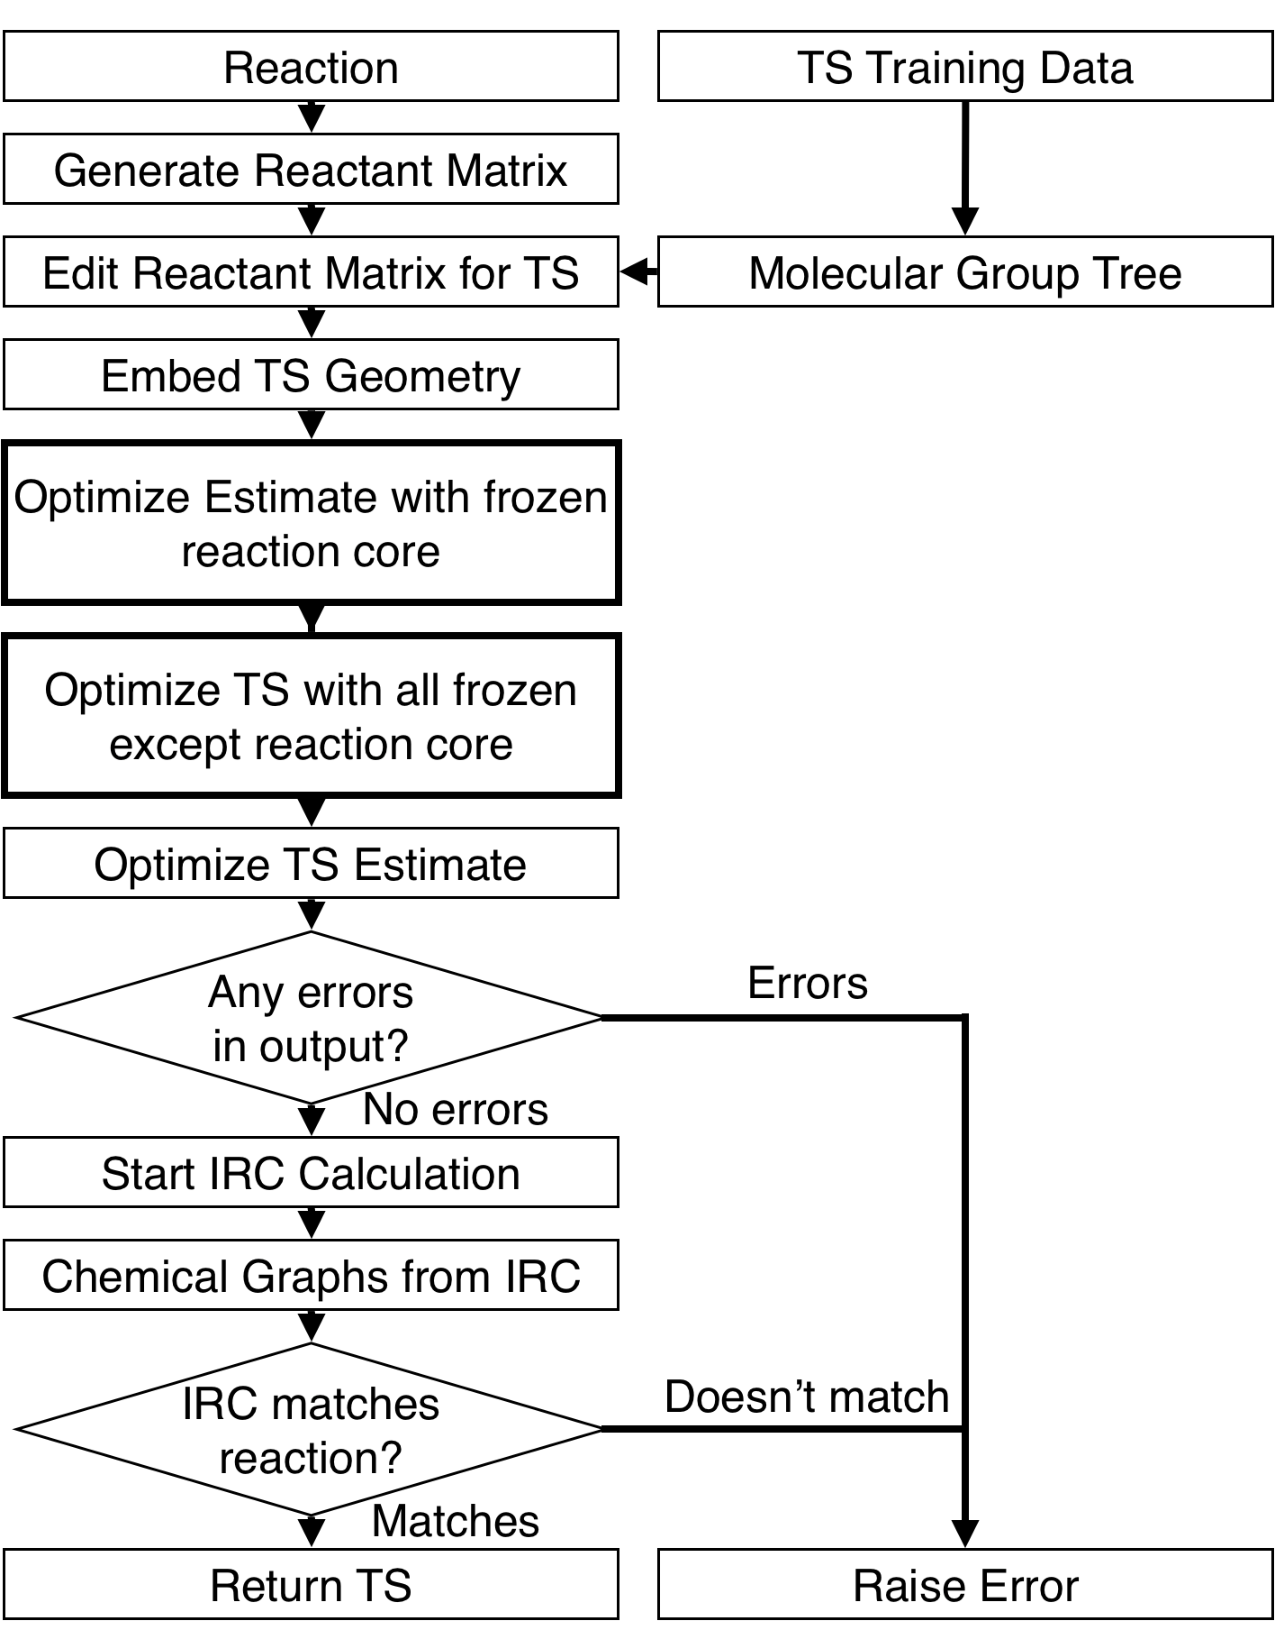
\includegraphics[width=0.4\textwidth]{autotst_overview}
    \caption{A flow chart describing the workflow of AutoTST, modified from \cite{bhoorasingh:2017}.}
    \label{fig:autotst_overview}
\end{figure}


%With these key distances, AutoTST then employees RDKit \cite{RDKit:2018} to generate three-dimensional geometries of reactant, product, and TS geometries.
%Reactant and product geometries are created using RDKit's built-in embed feature at an L0 level of theory. 
%A bounds matrix describing upper and lower allowable distances between atoms is generated for TS geometries and the distances between reacting atoms are set according to key distances.
%This matrix is used to generate a 3D geometry guess of the TS.

To test this work flow, Bhoorasingh and coworkers attempted calculations for 1117 reactions present in a model for the combustion of butanol and four of its isomers \cite{Sarathy:2012}, summarized in \tabref{table:ModelRxns}..
%Of these reactions, 885 were hydrogen abstraction reactions, 78 were intramolecular hydrogen migration reactions, and 184 were radical addition to multiple bond reactions. 
For each of these reaction families, AutoTST had success rates of approximately 70\%.

\begin{table}[h!]
\label{t:atst_r}
\small
\caption{\label{table:ModelRxns} Number of reactions for each family contained in the Sarathy et al. \cite{Sarathy:2012} combustion model and success of the AutoTST algorithm.}
\centering
\begin{tabular*}{\linewidth}{@{\extracolsep{\fill}}lccc}
\hline\rule{0pt}{2.6ex}%
Reaction Family & Number of  & Kinetics successfully & Percentage \\
  & Reactions  & calculated & calculated\\
\hline\rule{0pt}{2.6ex}%
Hydrogen abstraction & 855 & 598 & 70\% \\
Intramolecular hydrogen migration & 78 & 52 & 67\% \\
Radical addition to multiple bond & 184 & 131 & 71\% \\
\hline\rule{0pt}{2.6ex}%
Total & 1117 & 781 & 70\%\\
\hline
\end{tabular*}
\end{table}

A majority of AutoTST calculated kinetics agrees well with kinetics reported in the original model and estimates by RMG, but some had large disagreements with published kinetics. 
Bhoorasingh and co-workers commented that AutoTST's workflow would benefit from a detailed conformational analysis to find the correct low energy conformer, hindered rotor treatment for internal rotors, and a more accurate determination of symmetry numbers which is the focus of ongoing efforts. 


%%%%%%%%%%%%%%%%%%%%%%%%%%%%%%%%%%%%%%%%%%%%%%%%%%%%%%%%%%%%%%%%%%%%%%%%%%%%%%%%%%%%
%%%%%%%%%%%%%%%%%%%%%%%%%%%%%%%%%%%%%%%%%%%%%%%%%%%%%%%%%%%%%%%%%%%%%%%%%%%%%%%%%%%%
%%%%%%%%%%%%%%%%%%                                                %%%%%%%%%%%%%%%%%%
%%%%%%%%%%%%%%%%%%                     SC-AFIR                    %%%%%%%%%%%%%%%%%%
%%%%%%%%%%%%%%%%%%                                                %%%%%%%%%%%%%%%%%%
%%%%%%%%%%%%%%%%%%%%%%%%%%%%%%%%%%%%%%%%%%%%%%%%%%%%%%%%%%%%%%%%%%%%%%%%%%%%%%%%%%%%
%%%%%%%%%%%%%%%%%%%%%%%%%%%%%%%%%%%%%%%%%%%%%%%%%%%%%%%%%%%%%%%%%%%%%%%%%%%%%%%%%%%%

\subsection{AFIR (2016)}

The artificial force induced reaction (AFIR) is a code base that uses an artificial force to push or pull reacting fragments together or apart to find TSs \cite{Maeda:2016, Madea:2018}.\rhw{check bibliography for CAPITAL acronyms in titles. Wrap in \{\} to protect them} 

\begin{comment}
The artificial force applied is described by equation \eqnref{eq:afir}.
\rhw{all this about the forces seems too much detail to me, to understand the gist of the method}
\begin{equation}
    F^{AFIR}(\textbf{Q}) = E(\textbf{Q}) + \rho\alpha \frac{\sum_{i \in \textbf{A}} \sum_{j \in \textbf{B}} \omega_{ij}\textbf{\textit{r}}_{ij}}{\sum_{i \in \textbf{A}} \sum_{j \in \textbf{B}} \omega_{ij}}
    \label{eq:afir}
\end{equation}\rhw{the straightepsilon is undefined and thus missing. Check \LaTeX logs carefully for warnings and errors. (I think you meant $\in$ anyway)}

In the above equation, $E(\textbf{Q})$ is the PES of geometrical parameters $\textbf{Q}$, $\alpha$ is the strength of the force, $\rho$ is either 1.0 or -1.0, $r_{ij}$ is the interatomic distance between atoms $i$ and $j$, and $\omega_{ij}$ is defined using the below where $\textbf{\textit{R}}_i$ and $\textbf{\textit{R}}_j$ are the covalent radii of atoms $i$ and $j$.

\begin{equation}
    \omega_{ij} = \Big( \frac{\textbf{\textit{R}}_i + \textbf{\textit{R}}_j}{\textbf{\textit{r}}_{ij}} \Big)^6
\end{equation}

The force parameter is defined as follows.
In equation \eqnref{eq:alpha}, $\textit{R}_0$ and $\varepsilon$ are 3.8164~\AA\ \rhw{angstrom is undefined and thus missing. Check \LaTeX logs carefully for warnings and errors and fix them all. (in this case \AA)} and 1.0061~kJ/mol, respectively, and are parameters of the Lennard-Jones potential for the Ar-Ar interaction.
$\gamma$ represents the user defined collision energy and is used as an approximate upper limit of the barrier height for the system. 

\begin{equation}
    \alpha = \frac{\gamma}{\big[2^{-\frac{1}{6}} - \big( 1+ \sqrt{1+ \frac{\gamma}{\varepsilon }} \big)^{-\frac{1}{6}} \big] \textbf{\textit{R}}_0}
    \label{eq:alpha}
\end{equation}
\end{comment}

The AFIR method obtains a reaction path by minimizing the internal forces of a complex after an artificial force is applied.
This path is dependant on the initial structure and the reacting atoms chosen by the user. 
For example, AFIR will use single component (SC) and multi component (MC) artificial force methods for find reaction paths that correspond to unimolecular and multimolecular reactions, respectively.
In SC optimization, equidistant path points are first distributed along the reaction path and then stepped tangent to the reaction path and optimized.
This optimization is performed 10 times with a large step (1.0 \AA) and then five times with a small step (0.5 \AA). 
The minimum energy points correspond to the reactants and products and the maximum energy points correspond to TSs found. 
All geometries are then optimized by a standard quasi-Newton method and IRC calculations are performed to validate all identified TSs.

In the MC method, starting reactant geometries are either randomly generated or are provided by users and pushed together.
These starting geometries are used to find TSs by reacting fragments of the reaction complex and analyzing the reaction path.
In the SC method, fragments of a starting unimolecular reactant are pushed or pulled apart. 
These fragments include reacting atoms and atoms neighboring the reacting atoms noninclusive of atoms neighboring both reacting atoms.

AFIR methods have been used in a variety of studies \cite{Maeda:2016, Madea:2018} with Aldol reactions, Claisen rearrangements, and Co-catalyzed hydroformylation to name a few \cite{Maeda:2016}.
In addition, the AFIR method is a well-established method available in the GRRM17 software, an electronic structure code \cite{Madea:2013}.


%%%%%%%%%%%%%%%%%%%%%%%%%%%%%%%%%%%%%%%%%%%%%%%%%%%%%%%%%%%%%%%%%%%%%%%%%%%%%%%%%%%%
%%%%%%%%%%%%%%%%%%%%%%%%%%%%%%%%%%%%%%%%%%%%%%%%%%%%%%%%%%%%%%%%%%%%%%%%%%%%%%%%%%%%
%%%%%%%%%%%%%%%%%%                                                %%%%%%%%%%%%%%%%%%
%%%%%%%%%%%%%%%%%%                     AutoTS                     %%%%%%%%%%%%%%%%%%
%%%%%%%%%%%%%%%%%%                                                %%%%%%%%%%%%%%%%%%
%%%%%%%%%%%%%%%%%%%%%%%%%%%%%%%%%%%%%%%%%%%%%%%%%%%%%%%%%%%%%%%%%%%%%%%%%%%%%%%%%%%%
%%%%%%%%%%%%%%%%%%%%%%%%%%%%%%%%%%%%%%%%%%%%%%%%%%%%%%%%%%%%%%%%%%%%%%%%%%%%%%%%%%%%

\subsection{AutoTS (2017)}

AutoTS is a framework introduced by Jacobson et al. from Schr\"{o}dinger Inc. \cite{jacobson:2017}. 
This workflow is included in Jaguar version 9.7 \cite{Jaguar:2013},  a commercial quantum chemistry package provided by Schr\"{o}dinger Inc., and is shown in \figref{fig:autots_workflow}.

AutoTS requires users to provide geometries of the reactants and products at stable energy minima.
AutoTS determines reacting bonds and atom correspondence between reactants and products through an iterative bond deletion method by systematically breaking bonds, generating canonicalized SMILES strings for the modified reactant and product complexes, and comparing said strings.
The algorithm will first check if the complexes are identical, if not it will break one bond at a time.
If the complexes are not identical after deleting one bond at a time, the algorithm will break two at a time by systematically looping through all possible combinations of bonds.
This process will continue searching up to a default of four broken bonds.
Once changing bonds are identified, input geometries of reactant and product complexes are used to create the TS guess.

AutoTS can generate TS guesses by linear searches or by templating. 
A linear search will position reacting molecules at opposite corners of a cube with reacting atoms pointed towards each other at a distance large enough so molecules do not overlap.
The TS guess is created by calculating energies along a linear distance coordinate path connecting the reactants and products using an L2 level of theory.
Interpolation along cubic splines is used to identify the energy maximum geometry to be used as the starting TS guess.

Templating creates TS guesses by using ``templates''  from previously optimized TS geometries, stored in an auxiliary file containing geometries for successfully calculated TSs and string representations of the corresponding reactions.
Subgroup complexes are then generated of the $i$th order by including the ($i-1$)th neighboring atoms in the reaction center. 
If a match exists in the auxiliary file, the matching atoms are set to the corresponding atoms in the previously run TS and then optimized to a saddle point at a L2 level of theory.
%using quadratic synchronous transit and a quasi-Newton eigenvector at a L2 level of theory.

TSs are verified through two processes: ``vetting'' and ``connecting''. 
Vetting assesses if the TS meets three criteria: (1) there is exactly one imaginary frequency, (2) the TS geometry has at least one active bond at an intermediate distance, and (3) the translational mode corresponding to the imaginary frequency contains motion along an active bond.
If vetting is successful, the TS complex is connected by a modified three-point IRC calculation to identify reactant, TS, and product geometries. 
A TS is validated if connected to the input reactant and product geometries.
Although AutoTS has a robust method to find TSs, it does not return kinetic parameters, just thermodynamic parameters for reactant, product, and TS geometries.

\begin{figure}[htbp]
\centering
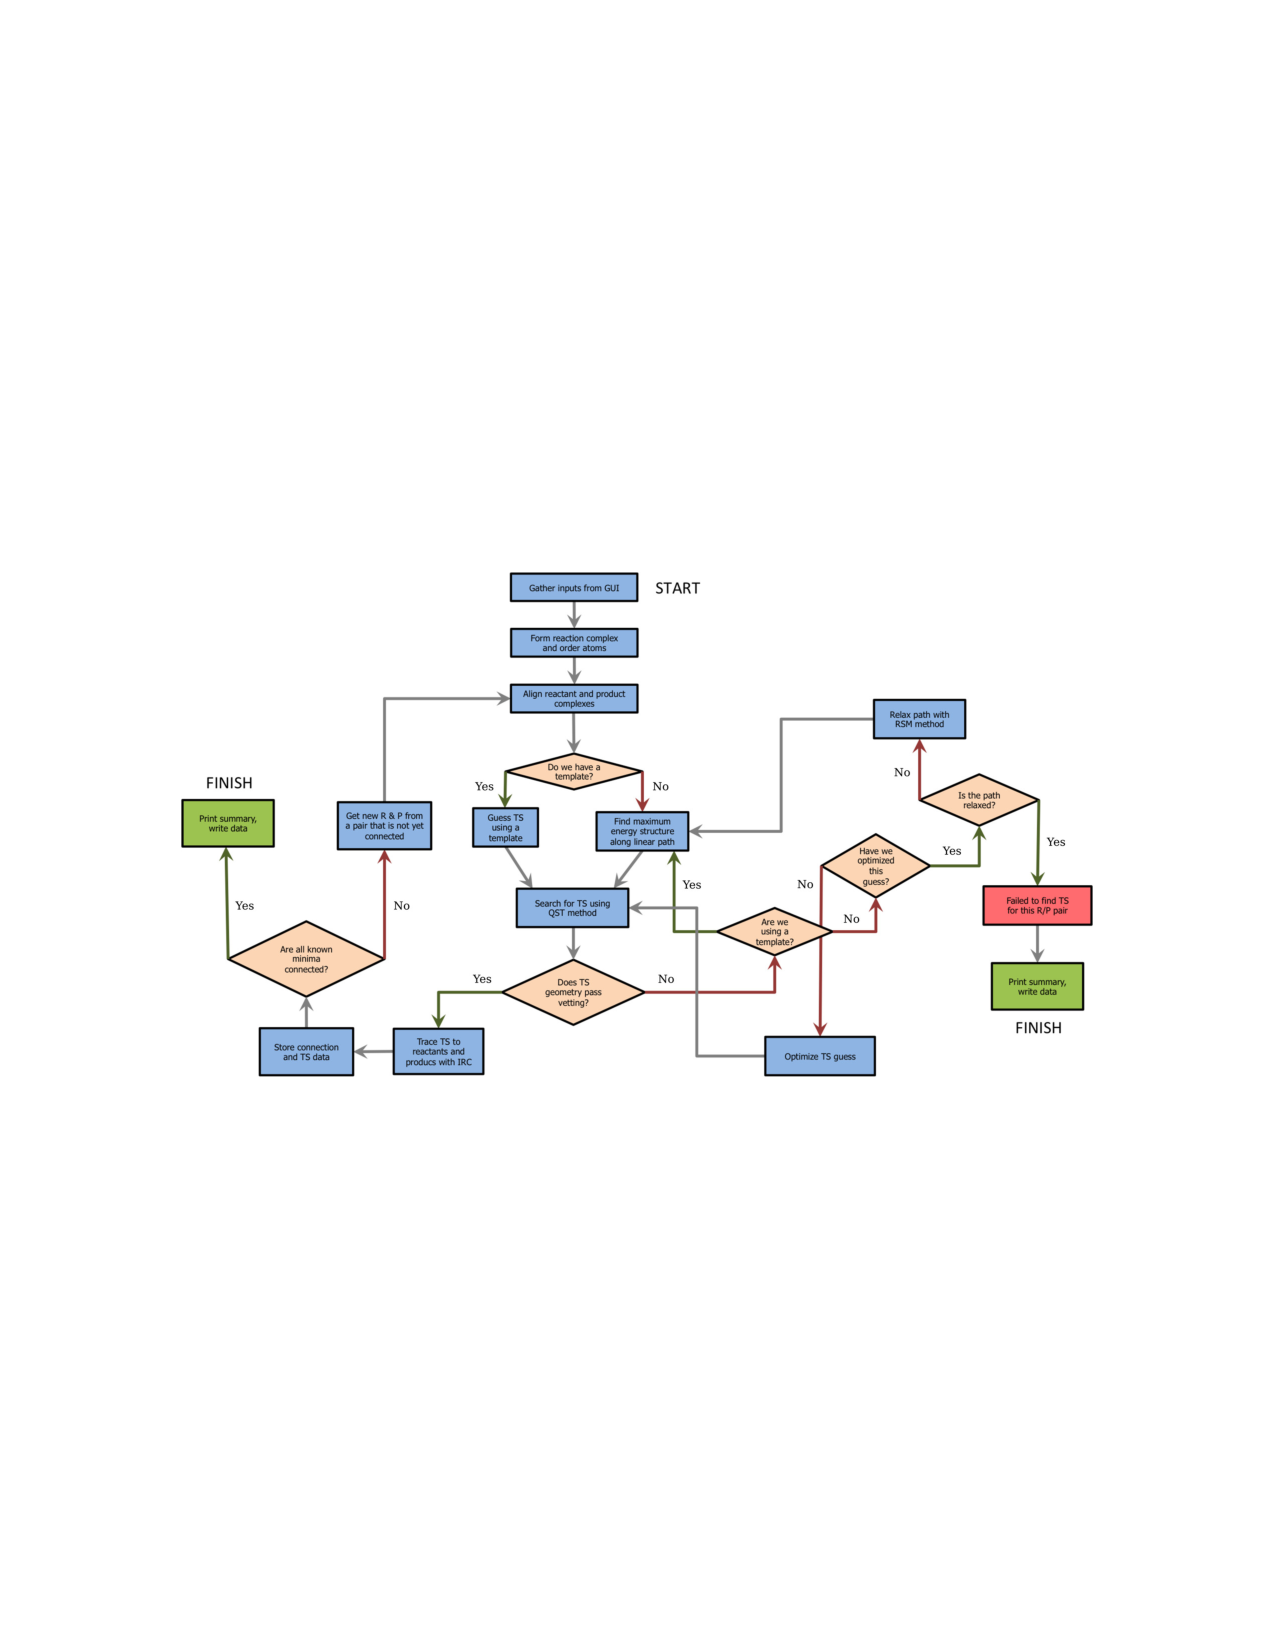
\includegraphics[width=\textwidth]{autots_workflow}
\caption{A flow diagram of AutoTS taken from \cite{jacobson:2017}. Input geometries are read and used generate TS guesses using templates or from linear interpolation. Fail-safes are in place to ensure all options are exhausted when finding the correct TS geometry.}
\label{fig:autots_workflow}
\end{figure}

To test the efficacy of AutoTS, Jacobson and coworkers used test sets for four reaction families: Michael addition, carbene insertion, hydrogen abstraction, and Diels-Alder.
AutoTS has shown great efficacy in these test cases, although the authors do highlight area of improvement.
From the version of AutoTS published, the authors wished to add support of reactions that do not involve changing covalent bonds, reactions with spectator molecules, reactions involving transition metals, reactions with cage-like geometries, sterocenters of reacting atoms, conformational analysis (this version of AutoTS currently uses only the input conformation of reactants and products to generate TS geometries), and very large molecules (300+ atoms).


%%%%%%%%%%%%%%%%%%%%%%%%%%%%%%%%%%%%%%%%%%%%%%%%%%%%%%%%%%%%%%%%%%%%%%%%%%%%%%%%%%%%
%%%%%%%%%%%%%%%%%%%%%%%%%%%%%%%%%%%%%%%%%%%%%%%%%%%%%%%%%%%%%%%%%%%%%%%%%%%%%%%%%%%%
%%%%%%%%%%%%%%%%%%                                                %%%%%%%%%%%%%%%%%%
%%%%%%%%%%%%%%%%%%                     GENESYS                    %%%%%%%%%%%%%%%%%%
%%%%%%%%%%%%%%%%%%                                                %%%%%%%%%%%%%%%%%%
%%%%%%%%%%%%%%%%%%%%%%%%%%%%%%%%%%%%%%%%%%%%%%%%%%%%%%%%%%%%%%%%%%%%%%%%%%%%%%%%%%%%
%%%%%%%%%%%%%%%%%%%%%%%%%%%%%%%%%%%%%%%%%%%%%%%%%%%%%%%%%%%%%%%%%%%%%%%%%%%%%%%%%%%%

\subsection{Genesys (2018)}

An automated TST calculator was recently added to Genesys, a reaction mechanism generator software developed by Vandewiele and co-workers at Ghent University \cite{VANDEVIJVER:2018, vandewiele:2012}.%, and is available through proprietary license. 
This tool requires users to provide a description of the reaction family, identify reacting atoms, and specification of quantum chemistry settings.
%A brief overview Genesys' work flow is given in \figref{fig:genesys_workflow}.

Reactant and product geometries are created by embedding using a L0 level of theory, followed by a rough geometry minimization at an L1 level of theory, and an exhaustive conformer analysis at a user defined level of theory (often at L1 or L2 level of theory).
Low energy conformers within a user defined specific cutoff criteria are identified and are further optimized at a user defined level of theory (often L2 level of theory).
After, the lowest energy conformer is used to attempt 1D hindered rotor scans on all rotatable bonds at a L2 level of theory.

TS complexes are generated by first matching the reaction to a template to identify reacting atoms.
Distances between reacting atoms are set to key distances that are based on previous TS searches or user specified.
Similar to AutoTST, 3D complexes are created by using the user specified key distances to create a 3D geometry at a L0 level of theory.
%editing the bounds matrix with the key distances and then embedded in a 3D geometry at a L0 level of theory.
Complexes are loosely optimized to a minima while keeping the reacting atoms fixed at a L1 level of theory.
TS geometries undergo exhaustive conformer searches at L1 or L2 user defined level of theory calculations by relaxing geometries to a minima, keeping the reaction center frozen.
The lowest energy conformer is optimized to a saddle point at a L2 level of theory where 1D hindered rotor scans are attempted. 
TSs are verified by identifying a only one imaginary frequency and calculating the change in bond lengths when applying Cartesian displacements of the imaginary frequency.
This is preformed in lieu of IRC calculations to reduce computational costs.
A TS is verified if the translational mode corresponding to the imaginary frequency contains motion along active bonds, and if these contributions are larger than that of the residual complex, the TS is validated. 
Validated TS, reactant, and product geometries are then used to extract Arrhenius parameters using statistical thermodynamics.
To test their workflow, the authors performed calculations on 8 reactions representative of the 8 supported reaction families and saw good agreement (within a factor of 2).

%%%%%%%%%%%%%%%%%%%%%%%%%%%%%%%%%%%%%%%%%%%%%%%%%%%%%%%%%%%%%%%%%%%%%%%%%%%%%%%%%%%%
%%%%%%%%%%%%%%%%%%%%%%%%%%%%%%%%%%%%%%%%%%%%%%%%%%%%%%%%%%%%%%%%%%%%%%%%%%%%%%%%%%%%
%%%%%%%%%%%%%%%%%%                                                %%%%%%%%%%%%%%%%%%
%%%%%%%%%%%%%%%%%%                     AARON                      %%%%%%%%%%%%%%%%%%
%%%%%%%%%%%%%%%%%%                                                %%%%%%%%%%%%%%%%%%
%%%%%%%%%%%%%%%%%%%%%%%%%%%%%%%%%%%%%%%%%%%%%%%%%%%%%%%%%%%%%%%%%%%%%%%%%%%%%%%%%%%%
%%%%%%%%%%%%%%%%%%%%%%%%%%%%%%%%%%%%%%%%%%%%%%%%%%%%%%%%%%%%%%%%%%%%%%%%%%%%%%%%%%%%

\subsection{AARON (2018)}

The open-source AARON code-base (An Automated Reaction Optimizer for New catalysts) is a software developed by Guan and co-workers to perform automated quantum mechanic calculations for catalytic reactions involving chiral products \cite{Guan:2018}. 
%AARON is freely available under the GPL-3.0 license.
A brief overview of the workflow is shown in \figref{fig:aaron_workflow}.
%AARON is built on the AaronTools \cite{aarontools:2018} collection which allows users to build and modify 3D geometries by reading in \texttt{.xyz} files.

\begin{figure}[htbp]
    \centering
    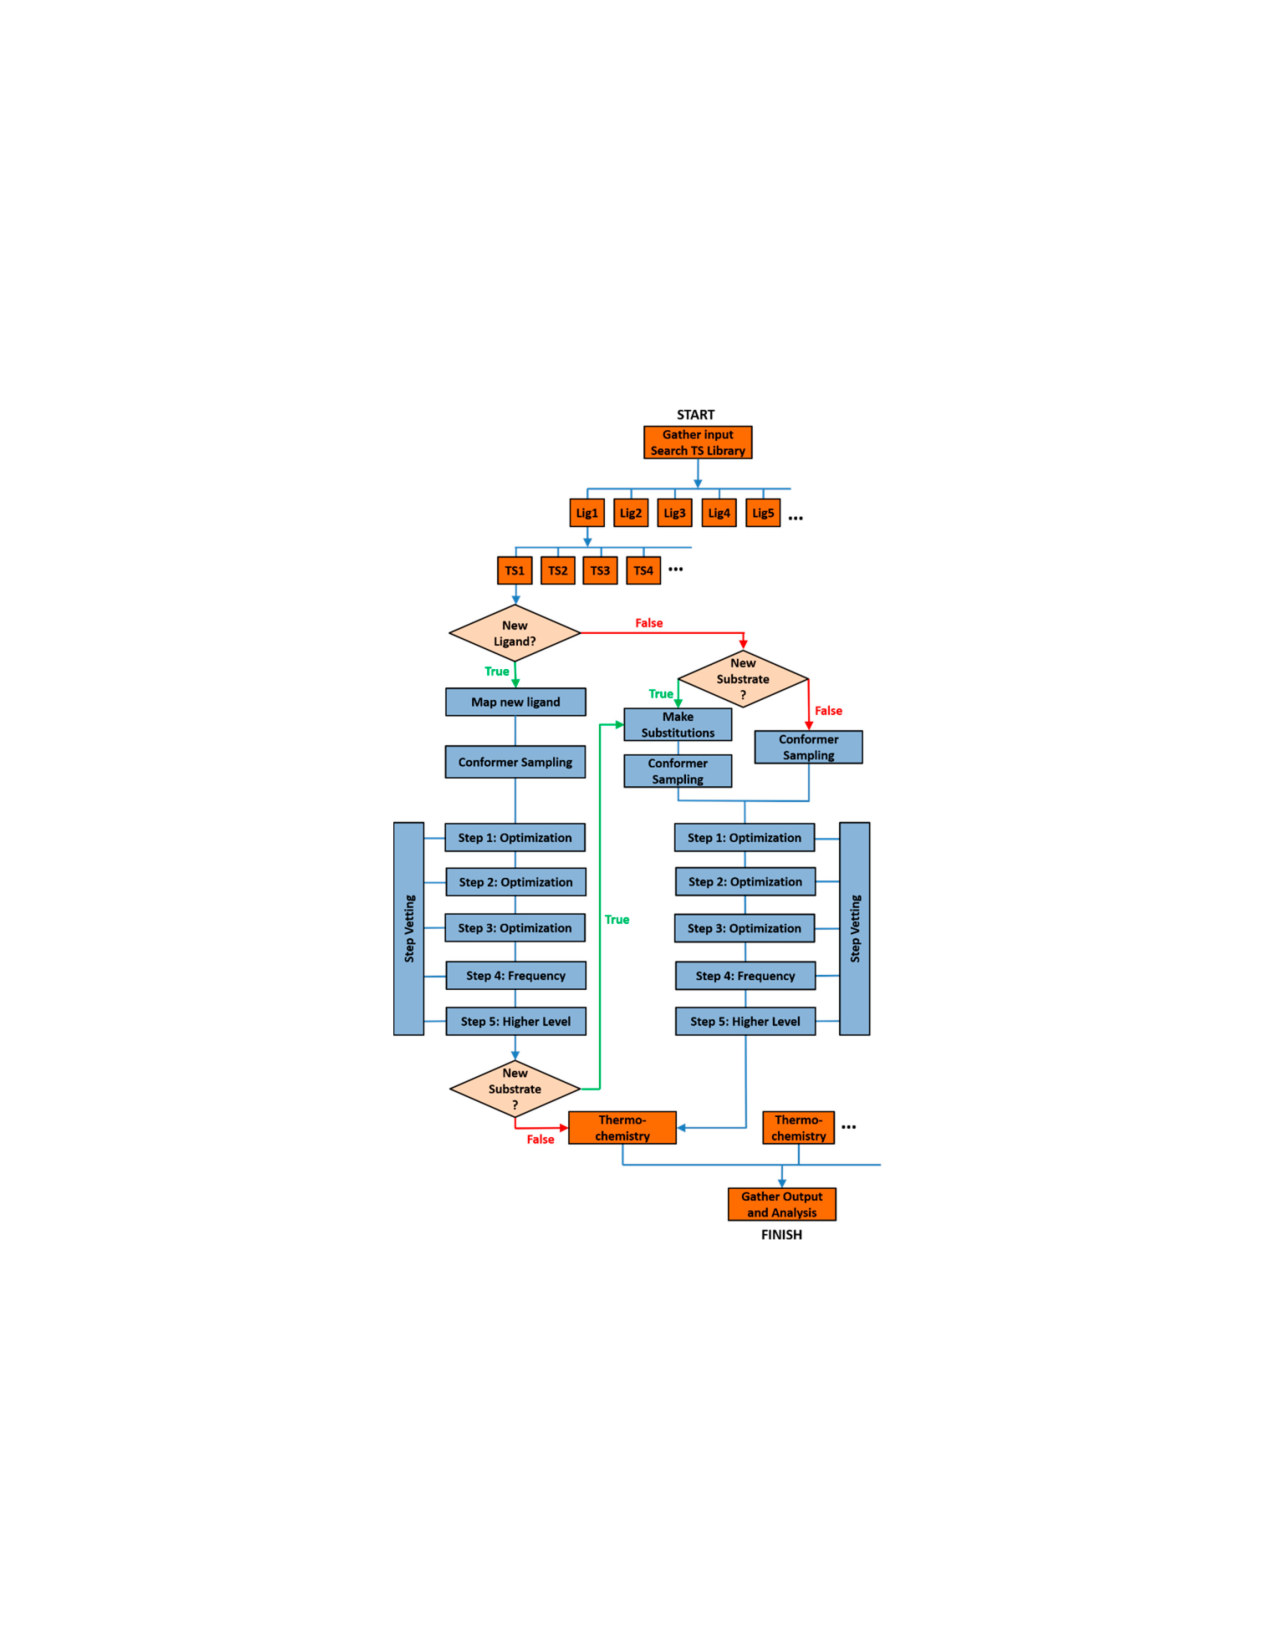
\includegraphics[width=0.3\textwidth]{aaron_workflow}
    \caption{An overview of the AARON workflow. Borrowed from \cite{Guan:2018}.}
    \label{fig:aaron_workflow}
\end{figure}

AARON generates TS guesses by having users provide input files containing reactant geometries and reactive atoms.
AARON requires a seed library containing previously optimized geometries for a family of interest and ``templates'' the reaction similarly to AutoTS.
This involves identifying a previous geometry that closely resembles the TS of interest, setting all similar atoms to positions of the previous geometry, and replacing non-similar atoms with their correct counterparts.
The TS guesses undergo a rule based conformer analysis investigating (1) conformers for substituents deemed ``new'' by AARON or the user, (2) torsional angles based off the symmetry of the dihedral, and (3) ``generations'' of conformers evaluated hierarchically.
For the hierarchical search, the first ``generation'' of conformers are created by rotating a single torsions and optimizing to generate unique conformers.
The next torsions of these unique conformers are rotated and optimized to create children for the next generation. 
If an optimized child is a duplicate of a previously identified conformer, it is not used to create future generations.
This process repeats until all torsions have been evaluated. 
Unique conformers are used in a Boltzmann-weighted sum to determine thermochemical parameters of TS complexes. 

AARON also implements an error handling workflow called ``Step Vetting'' to solve problems that arise and to validate TS geometries.%, a diagram is given in \figref{fig:aaron_exception}.
Step Vetting will follow geometries through the workflow to check for and attempt to correct common errors (e.g. breaking of non-reactive bonds, atoms clashing, and more).

\begin{comment}
\begin{figure}[htbp]
    \centering
    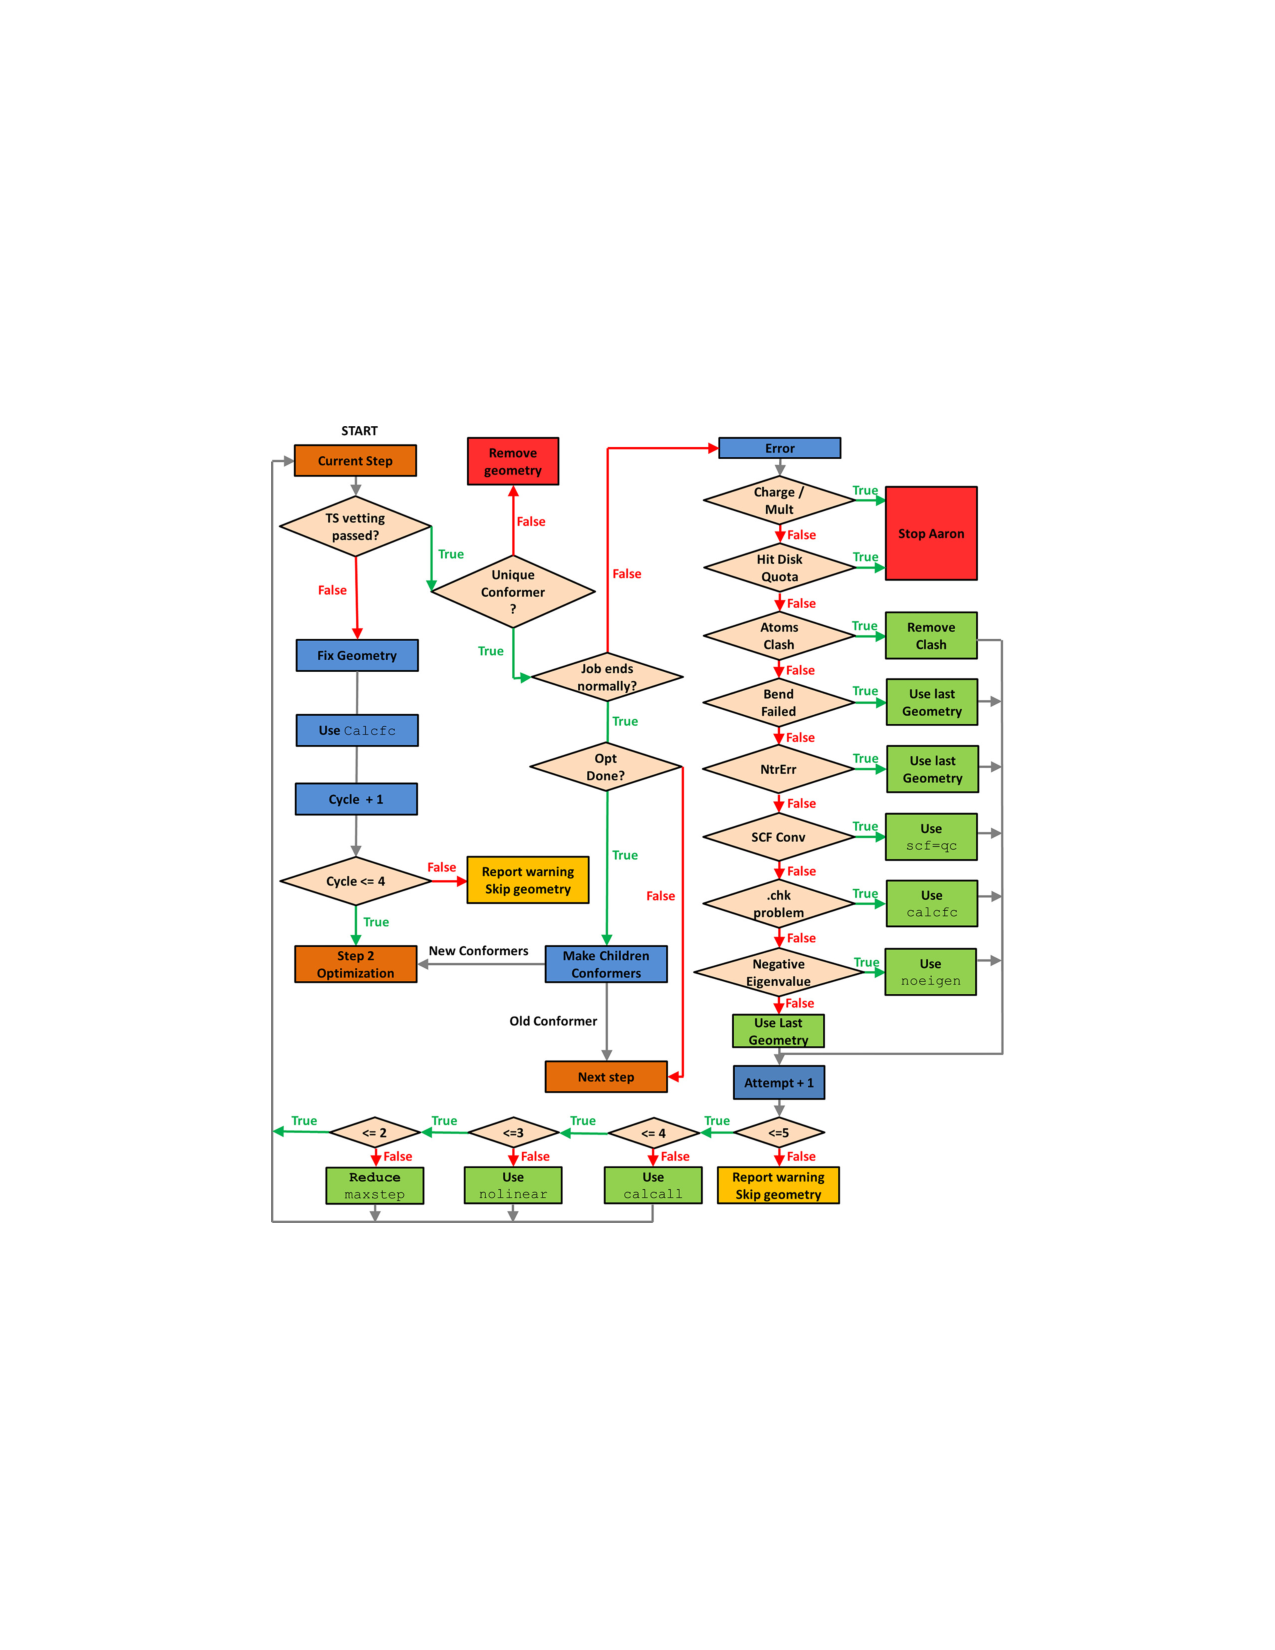
\includegraphics[width=\textwidth]{aaron_exception}
    \caption{The procedure for ``Step Vetting'' used in AARON to monitor jobs when searching for TS geometries.}
    \label{fig:aaron_exception}
\end{figure}
\end{comment}

To test this workflow, the authors looked at three test sets: Pd-catalyzed Heck allenylation, Rh-catalyzed hydrogenation of enamides, and Lewis-base promoted propargylation of aromatic aldehydes.
In each test case, small template libraries were created using a published set of TS geometries used by AARON to perform TS searches using Gaussian \cite{Gaussian:2009}.
AARON was able to locate a majority of the TS geometries with good agreement in energies.
While still in its early stages of development, AARON can be improved by implementing an automated approach to create TS libraries by making use of the TS data generated during each run.


%s\begin{equation}
%    \gamma = -R T\ln\Big(\frac{h}{t k_B T}\Big)
%\end{equation}

%%%%%%%%%%%%%%%%%%%%%%%%%%%%%%%%%%%%%%%%%%%%%%%%%%%%%%%%%%%%%%%%%%%%%%%%%%%%%%%%%%%%
%%%%%%%%%%%%%%%%%%%%%%%%%%%%%%%%%%%%%%%%%%%%%%%%%%%%%%%%%%%%%%%%%%%%%%%%%%%%%%%%%%%%
%%%%%%%%%%%%%%%%%%                                                %%%%%%%%%%%%%%%%%%
%%%%%%%%%%%%%%%%%%                    EStokTP                     %%%%%%%%%%%%%%%%%%
%%%%%%%%%%%%%%%%%%                                                %%%%%%%%%%%%%%%%%%
%%%%%%%%%%%%%%%%%%%%%%%%%%%%%%%%%%%%%%%%%%%%%%%%%%%%%%%%%%%%%%%%%%%%%%%%%%%%%%%%%%%%
%%%%%%%%%%%%%%%%%%%%%%%%%%%%%%%%%%%%%%%%%%%%%%%%%%%%%%%%%%%%%%%%%%%%%%%%%%%%%%%%%%%%


\subsection{EStokTP (2018)}


EStokTP (Electronic Structure to k(T,P)) \cite{Cavallotti:2019jctc} is an automated rate calculator by Cavallotti and Klippenstein that returns a temperature, a pressure dependent rate constant expression, and optimized electronic structures of reactants, products, and TSs.
A general program structure for abstraction reactions in EStokTP is shown in \figref{fig:estoktp_structure}.
%EStokTP is freely available under the GPL-3.0 liscense.

A user will provide the desired quantum methods, a reasonable guesses for some internal coordinates, and labeled atoms describing the reaction family to perform calculations.
Currently, EStokTP works for four reaction families: abstraction, addition, beta scission, and isomerization. 
%In the case of hydrogen abstraction inputs (shown in \figref{fig:estoktp_habstraction}), the user specifies the hydrogen being abstracted (\texttt{isite}), the atom bound to that hydrogen (\texttt{jsite}), and another atom connected to \texttt{jsite} (\texttt{ksite}).
%In addition, a dummy atom (X) is added to the complex as a reference point for atoms in the reaction center.
Users will then specify two entry angles for reactants and three dihedral angles between reacting atoms.
%These dihedral angles are as follows: first atom of abstracting reactant, \texttt{isite}, dummy atom, \texttt{jsite}; second atom of abstracting reactant, first atom of abstracting reactant, \texttt{isite}, dummy atom; and, (if available) third atom of abstracting reactant, second atom of abstracting reactant, first atom of abstracting reactant, \texttt{isite}.
EStokTP interfaces with Gaussian \cite{Gaussian:2009} or MolPro \cite{molpro:2012} to construct the TS guess by positioning the reactants using the user specified internal coordinates. 
EStokTP will perform a conformer analysis by generating $5 + 3^n$ or $100$ TS conformers randomly, whichever is smaller, where $n$ is the number of non-methyl torsions. 
These conformers are relaxed and the highest energy geometry undergoes a series of partial optimizations to arrive at a saddle point at a L2 level of theory. 
The TS is validated through IRC calculations, and 1-, 2-, or 3D hindered rotor calculations are performed at a L2 level of theory.
Single point energies are calculated at a L3 level of theory.

EStokTP is unique in that it uses a multi van der Waals well method when identifying TS geometries and kinetics.
Van der Waals wells can be considered for both the reactant and product side (present in abstraction reactions), just the reactant side (present in addition and scission reaction), or not consider the van der Waals wells at all (in isomerization).
Reactant, product, and TS geometries are passed to MESS \cite{MESS:2013} to obtain kinetic parameters.


\begin{figure}[htbp]
    \centering
    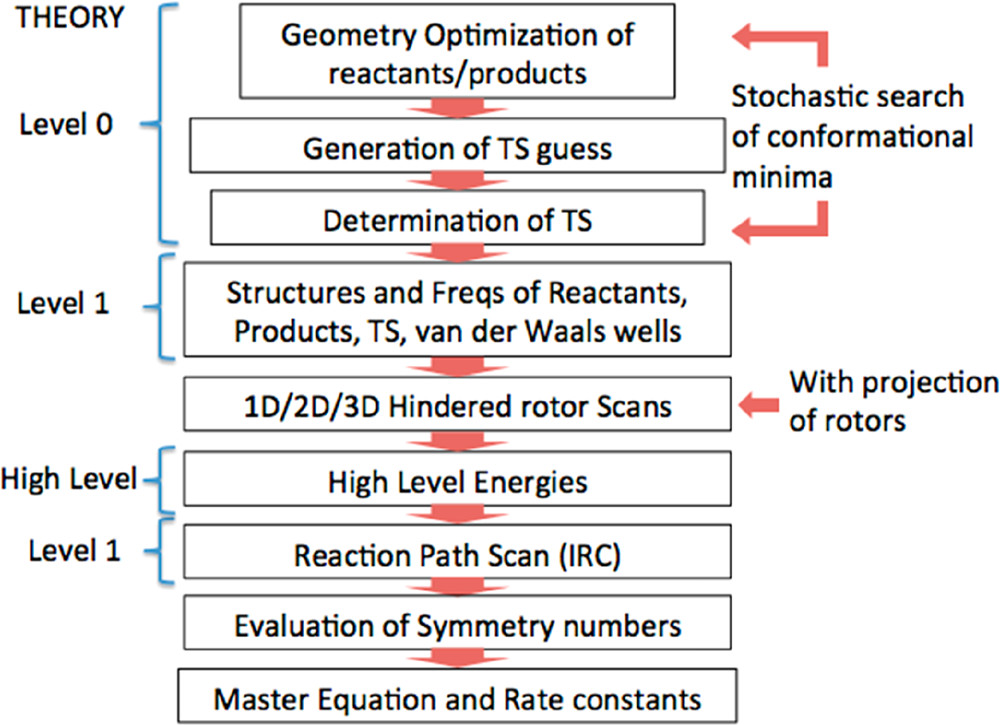
\includegraphics[width=0.5\textwidth]{estoktp}
    \caption{Program structure of EStokTP for abstraction reactions. Borrowed from \cite{Cavallotti:2019jctc}}
    \label{fig:estoktp_structure}
\end{figure}

\begin{comment}
\begin{figure}[htbp]
    \centering
    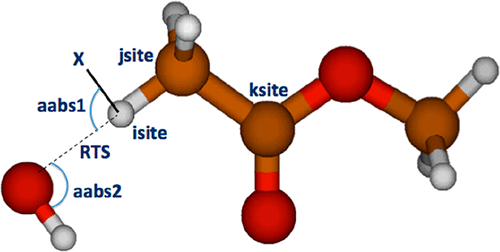
\includegraphics[width=0.5\textwidth]{estoktp_habstraction}
    \caption{TS geometry constructed for H abstraction in the \ce{OH} + methylacetate reaction. Specified  Figure from \cite{estoktp:2018}}
    \label{fig:estoktp_habstraction}
    \rhw[inline]{reduce figure size. are those blue text bits needed or mentioned? does the figure help?}
\end{figure}
\end{comment}


Cavollotti and co-workers studied test sets of hydrogen abstraction and addition reactions, and discussed EStokTP's is ablity to perform calculations on isomerization, beta-scission, barrierless, and multiple well reactions as well.
Although the methodology for barrierless reactions is promising, these reactions would benefit from variable reaction coordinate TST to accurately describe the translational modes.


%%%%%%%%%%%%%%%%%%%%%%%%%%%%%%%%%%%%%%%%%%%%%%%%%%%%%%%%%%%%%%%%%%%%%%%%%%%%%%%%%%%%
%%%%%%%%%%%%%%%%%%%%%%%%%%%%%%%%%%%%%%%%%%%%%%%%%%%%%%%%%%%%%%%%%%%%%%%%%%%%%%%%%%%%
%%%%%%%%%%%%%%%%%%                                                %%%%%%%%%%%%%%%%%%
%%%%%%%%%%%%%%%%%%                     KinBot                     %%%%%%%%%%%%%%%%%%
%%%%%%%%%%%%%%%%%%                                                %%%%%%%%%%%%%%%%%%
%%%%%%%%%%%%%%%%%%%%%%%%%%%%%%%%%%%%%%%%%%%%%%%%%%%%%%%%%%%%%%%%%%%%%%%%%%%%%%%%%%%%
%%%%%%%%%%%%%%%%%%%%%%%%%%%%%%%%%%%%%%%%%%%%%%%%%%%%%%%%%%%%%%%%%%%%%%%%%%%%%%%%%%%%

\subsection{KinBot (2019)}


KinBot \cite{kinbot:2018, kinbot:2019}, developed by Z\'{a}dor and co-workers at Sandia National Labs, crosses the bridge between reaction mechanism generation, automatic TST calculations, and PES exploration.
Because this review focuses on TST, reference the recent publication by Van de Vijver and Z\'{a}dor for a detailed description of KinBot's PES exploration methods \cite{kinbot:2019}.
%KinBot is freely available through the BSD 3-Clause liscense.

Kinbot investigates TS geometries for all possible reactions a species can undergo (i.e. rather than investigating a single reaction, Kinbot evaluates many).
To run KinBot, a user provides the structure of the species of interest (via SMILES string or Cartesian coordinates), its multiplicity, quantum methods, and reaction families to investigate. 
KinBot first performs a systematic or random conformational search and a geometry optimization of the reactant geometries using the Gaussian quantum chemistry suite.
By default, a systematic conformer search will be performed and it will iterate through all rotatable torsions and orientations of cyclic substructures. 
Conformers are then optimized at a L1 level of theory to identify the lowest energy conformer, which is then optimized to calculate frequencies at a L2 level of theory.
If the reactant provided contains many rotatable bonds, a user may specify a maximum number of samples to use during a calculation and to use a random sampling mechanism rather than the default.
To ensure the lowest energy conformer is isomorphic to the starting species and TSs, KinBot will ensure no bond lengths significantly change, resulting in unwanted rearrangements of atoms.

\begin{comment}
\begin{figure}[htbp]
    \centering
    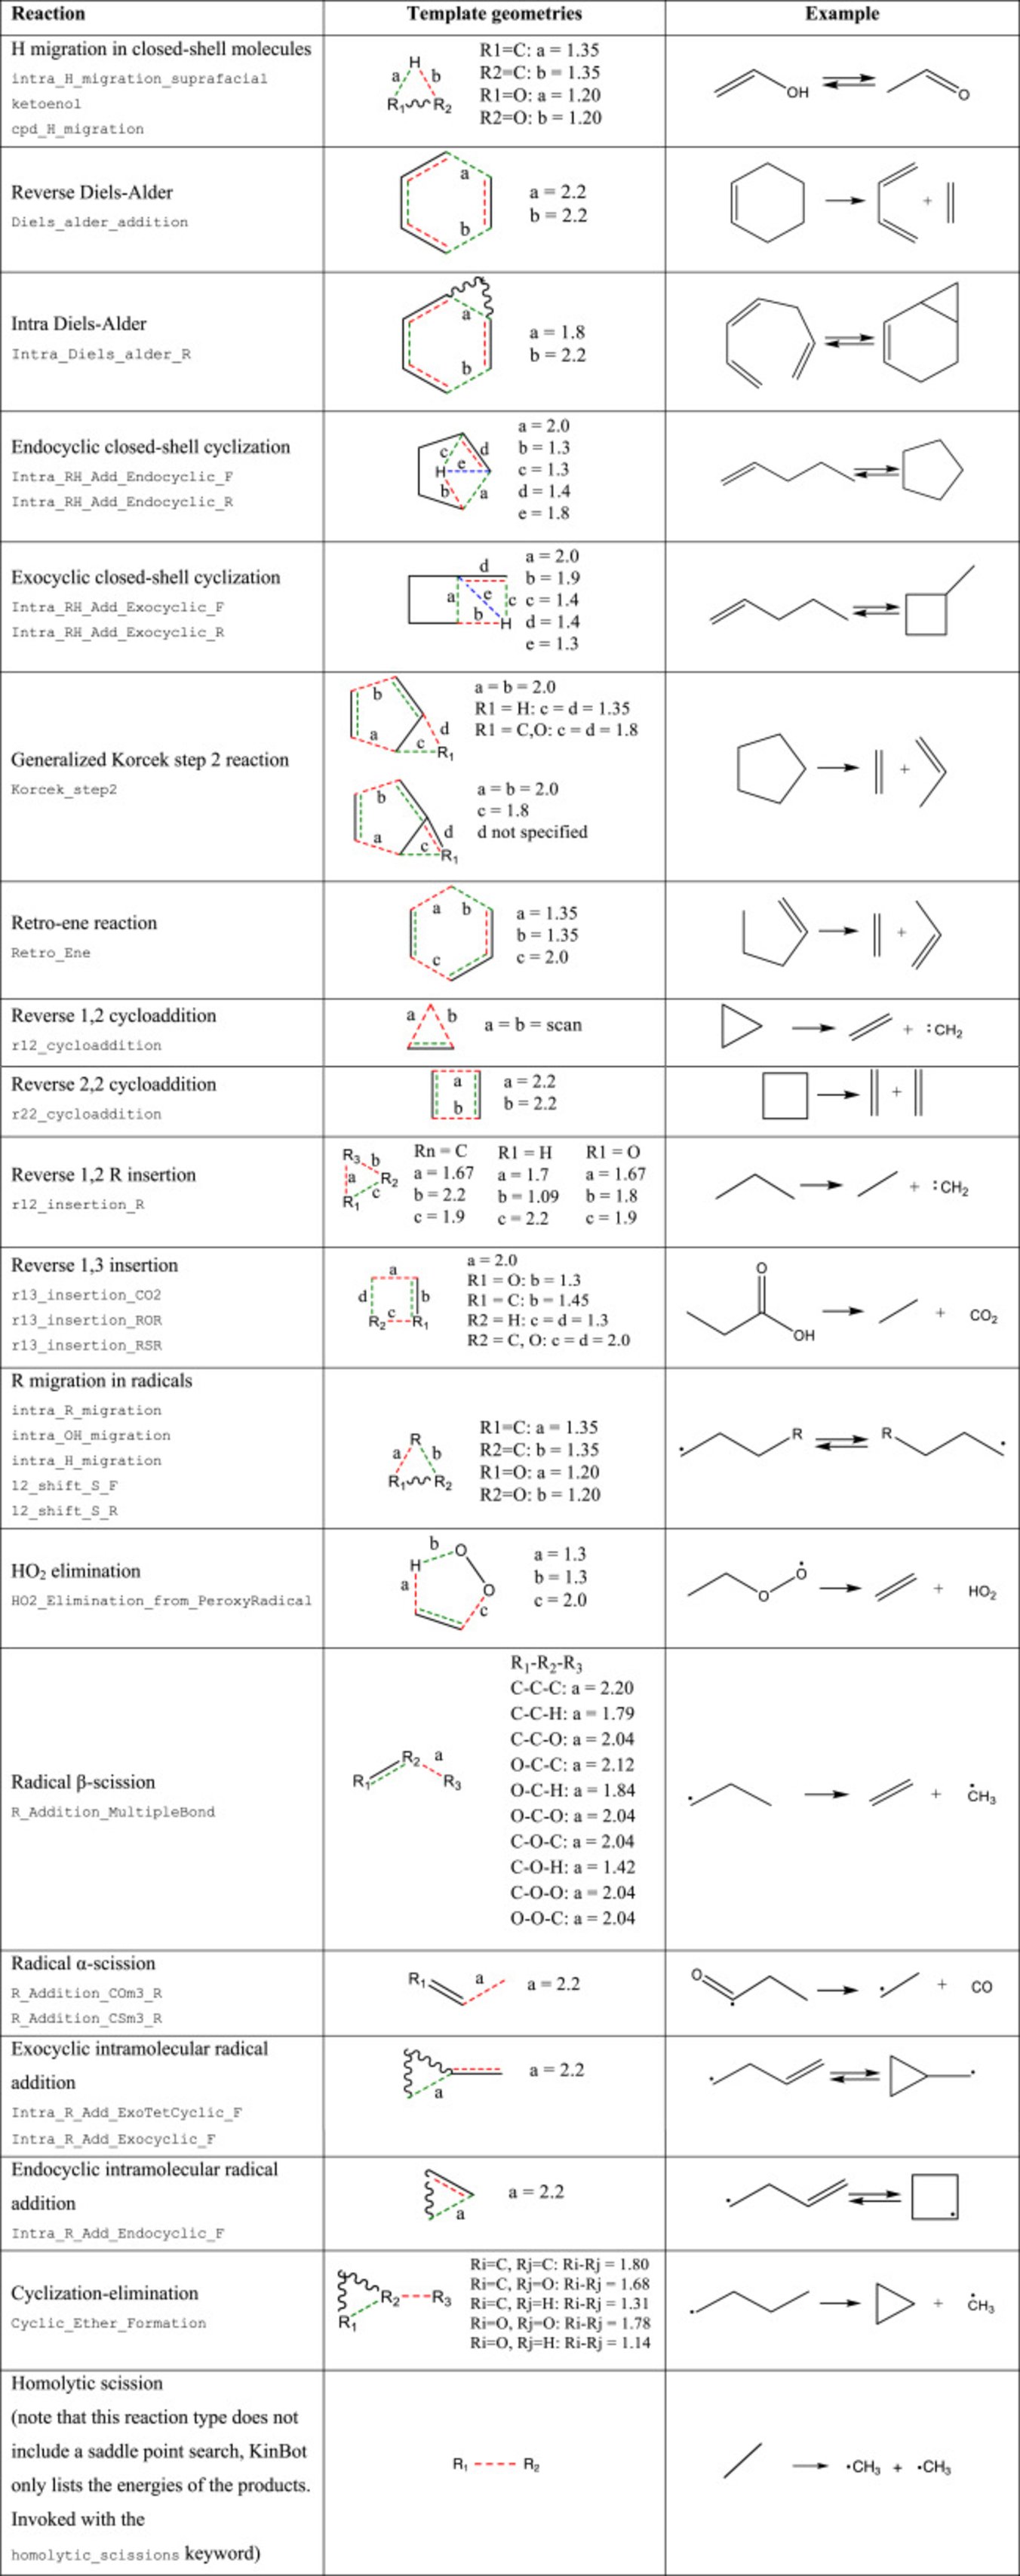
\includegraphics[width=0.5\textwidth]{kinbot_reactions}
    \caption{A table describing all of the reaction families supported by KinBot, from \cite{kinbot:2019}.}
    \label{fig:kinbot_families}
    \rhw[inline]{maybe we leave out the full table (refer to original publication) or list them somehow?}
\end{figure}
\end{comment}

KinBot relies on predefined reaction families, or general reaction templates, when generating mechanisms. 
From a user specified list of reaction families (described in \cite{kinbot:2019}), KinBot will set up a TS guess using either a ``direct'', ``indirect'', or ``scan'' strategy performed at a low level of theory (L0).
Through the direct and indirect methods, a TS guess is created by performing a series of geometry modifications and constrained optimizations to bring reacting atoms to a specified distance. 
Torsions, angles, and bonds of the complex are modified (in that order) and undergo a constrained optimization with modified geometry frozen.
Alternatively, KinBot can use a scan method, where the TS guess is created by scanning the electronic energies along the active bond and selecting the maximum energy complex.

Once a TS guess is identified, the geometry is optimized to a first-order saddle point with a L1 level of theory, and if a saddle point is found, the geometry is optimized again and the frequencies are calculated at a L2 level of theory.
TS geometries are validated by IRC calculations and by asserting (1) that resultant reactants match the input reactants and (2) the product side of the geometry results in a product structure different than the input geometry generated by KinBot (e.g. \ce{A <=> A} isn't the resultant reaction).
Once TS and product geometries are found, a conformer analysis is performed identical to the reactants; however, TS geometries require special treatment. 
The TS conformer analysis will identify active bonds by comparing reactants and products when creating complexes and use them as conformational degrees of freedom.
Cyclic TSs are considered to be rings when performing conformational analysis.

Once reactant, product, and TS geometries are identified, internal rotors are scanned (if user requested) at a L2 level of theory.
KinBot systematically scans each rotatable dihedral in \ang{30} increments to be used in master equation codes to account for hindered rotations.
Additionally, if a lower energy conformer is identified while performing said scans, the scan restarts with the new lower energy conformer.

%\begin{equation}
%    V = \Sigma^{6}_{i=1} V_{ci}(1 - \cos(i \cdot \phi)) + \Sigma^{6}_{i=1} V_{si} \sin(i \cdot \phi)
%    \label{eq:hinderedrotor_kinbot}
%\end{equation}

Next, KinBot determines the symmetry number of reactants, products, and TS geometries using a set of rules based on atom, bond, and cycle contributions.
This is described in more detail in their recent publication \cite{kinbot:2019}.

\begin{comment}
KinBot will first iterate through atoms not present in a ring, will identify the number of neighbors and equivalent neighbors for each atom, and determine the each atom's contribution to the external symmetry using a tabular method.
Then it will iterate through all bonds and linear structures (\ce{C=C=C}) and, if the terminal atoms on either end of the bond or structure are equivalent, the external symmetry is increased by a factor of two.
In addition, if neighbors of the terminal atoms are equivalent, the external symmetry is increased depending on the equivalence.
Rings are broken at a bond to create a vector based on atom type and indexes, and this vector is ``rolled'' by shifting atom indexes by 1 while maintaining the order and is repeated to create all possible vectors.
This process is also repeated in the reverse direction (e.g. if the first vector created for a 6 member ring has indexes [1, 2, 3, 4, 5, 6] the reverse vector would be [1, 6, 5, 4, 3, 2]).
The reverse vector is also ``rolled'' and all possible vectors are stored.
At this point, the number of vectors that are atom type identical to the initial forward vector are counted and defined as $n$ and the ring contribution to the symmetry is defined as $n+1$. \ndh{is this too much detail?}
\end{comment}

Finally, KinBot (at the users request) performs single point energy calculations at a L3 level of theory.
All calculations performed by KinBot are able to be used in two master equation codes: MESS \cite{MESS:2013} or MESMER \cite{MESMER:2012}, where only minor manual input is required to perform rate estimations.

Van de Vijver and Zador tested the efficacy of KinBot on four different test sets: [1,3]-sigmatropic H-migration reactions, thermal decomposition of gamma-valerolactone, propene and OH, and Aramco Mech up to C4 species.
The authors do not comment on improvement in the article itself.


\subsection{TS Gen (2020)}

TS Gen is a machine learning based approach to calculate TS geometries developed by Grambow, Pattanaik, and co-workers \cite{grambow:2020, pattanaik:2020}.
A graphical representation of the workflow is shown in \figref{fig:ts_gen}.

\begin{figure}[htbp]
    \centering
    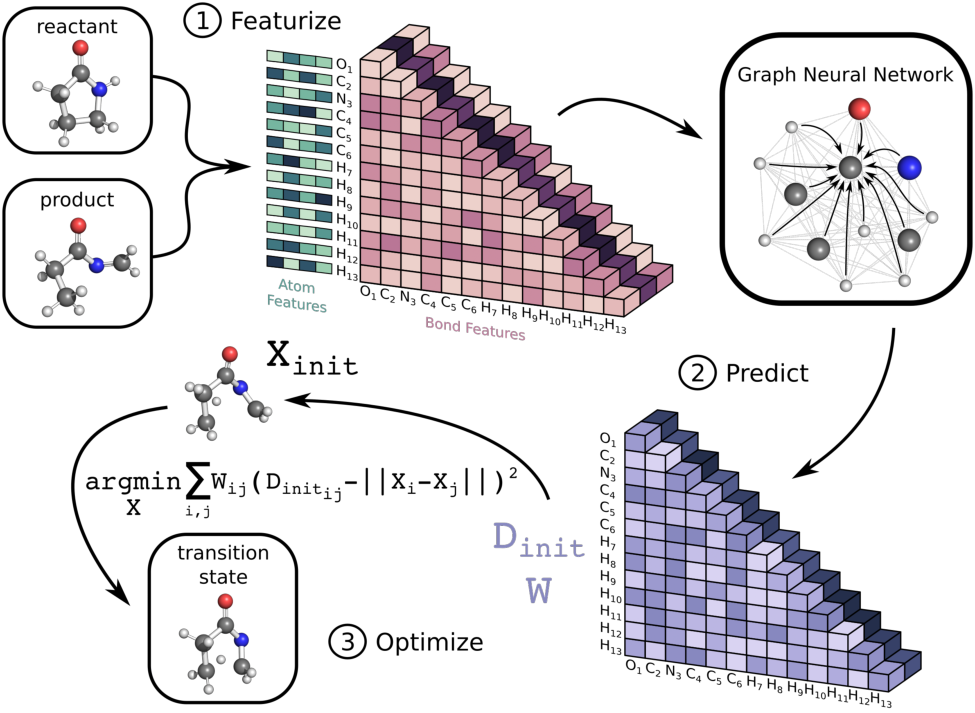
\includegraphics{ts-gen}
    \caption{Graphical representation of the workflow used in TS Gen borrowed from \cite{pattanaik:2020}.}
    \label{fig:ts_gen}
\end{figure}

TS Gen will start by creating a graphical representation of the TS structure by using reactant and product geometries.
This TS graph is fed into a graph neural network that generates an new representation of the TS graph.
The updated graph is fed into an additional dense layer of the network to generate a prediction of the pairwise distances between atoms ($D_{init}$ in \figref{fig:ts_gen}) and the weights describing the importance of those distances ($W$ in \figref{fig:ts_gen}) that will be used in a nonlinear least square (NLS) optimization.
The NSL optimization will minimize the residual between $D_init$ and the pairwise distances in the final coordinates of the TS, $X$, using \eqnref{eq:ts_gen}.

\begin{equation}
    \argmin_X \sum\limits_{ij} W_{ij} ( D_{init_{ij}} - || X_i - X_j ||)^2
    \label{eq:ts_gen}
\end{equation}
This optimization will then be used as the starting point for a single TS optimization using Gaussian \cite{Gaussian:2009}.

Once a first-order saddle point has been found, it is verified by checking that there is exactly one imaginary frequency and by performing an IRC calculation.
The IRC calculation is validated by reading in the output reactant and product geometries, optimizing to an energy minimum, and converting into graphs using Open Babel \cite{openbabel:2011} to check for isomorphism between input reactants and products.

The graph neural network was trained on approximately 1000 unique reactants and 8500 unimolecular isomerization reactions, split 80:10:10 for training, validation, and testing, respectively.
When comparing to the testing set, the NSL optimized TS geometries from trained graph neural network showed excellent agreement with the testing data (``Final Model'' vs. ``Ground Truth'' in \figref{fig:ml_agreement}). 

\begin{figure}[htbp]
    \centering
    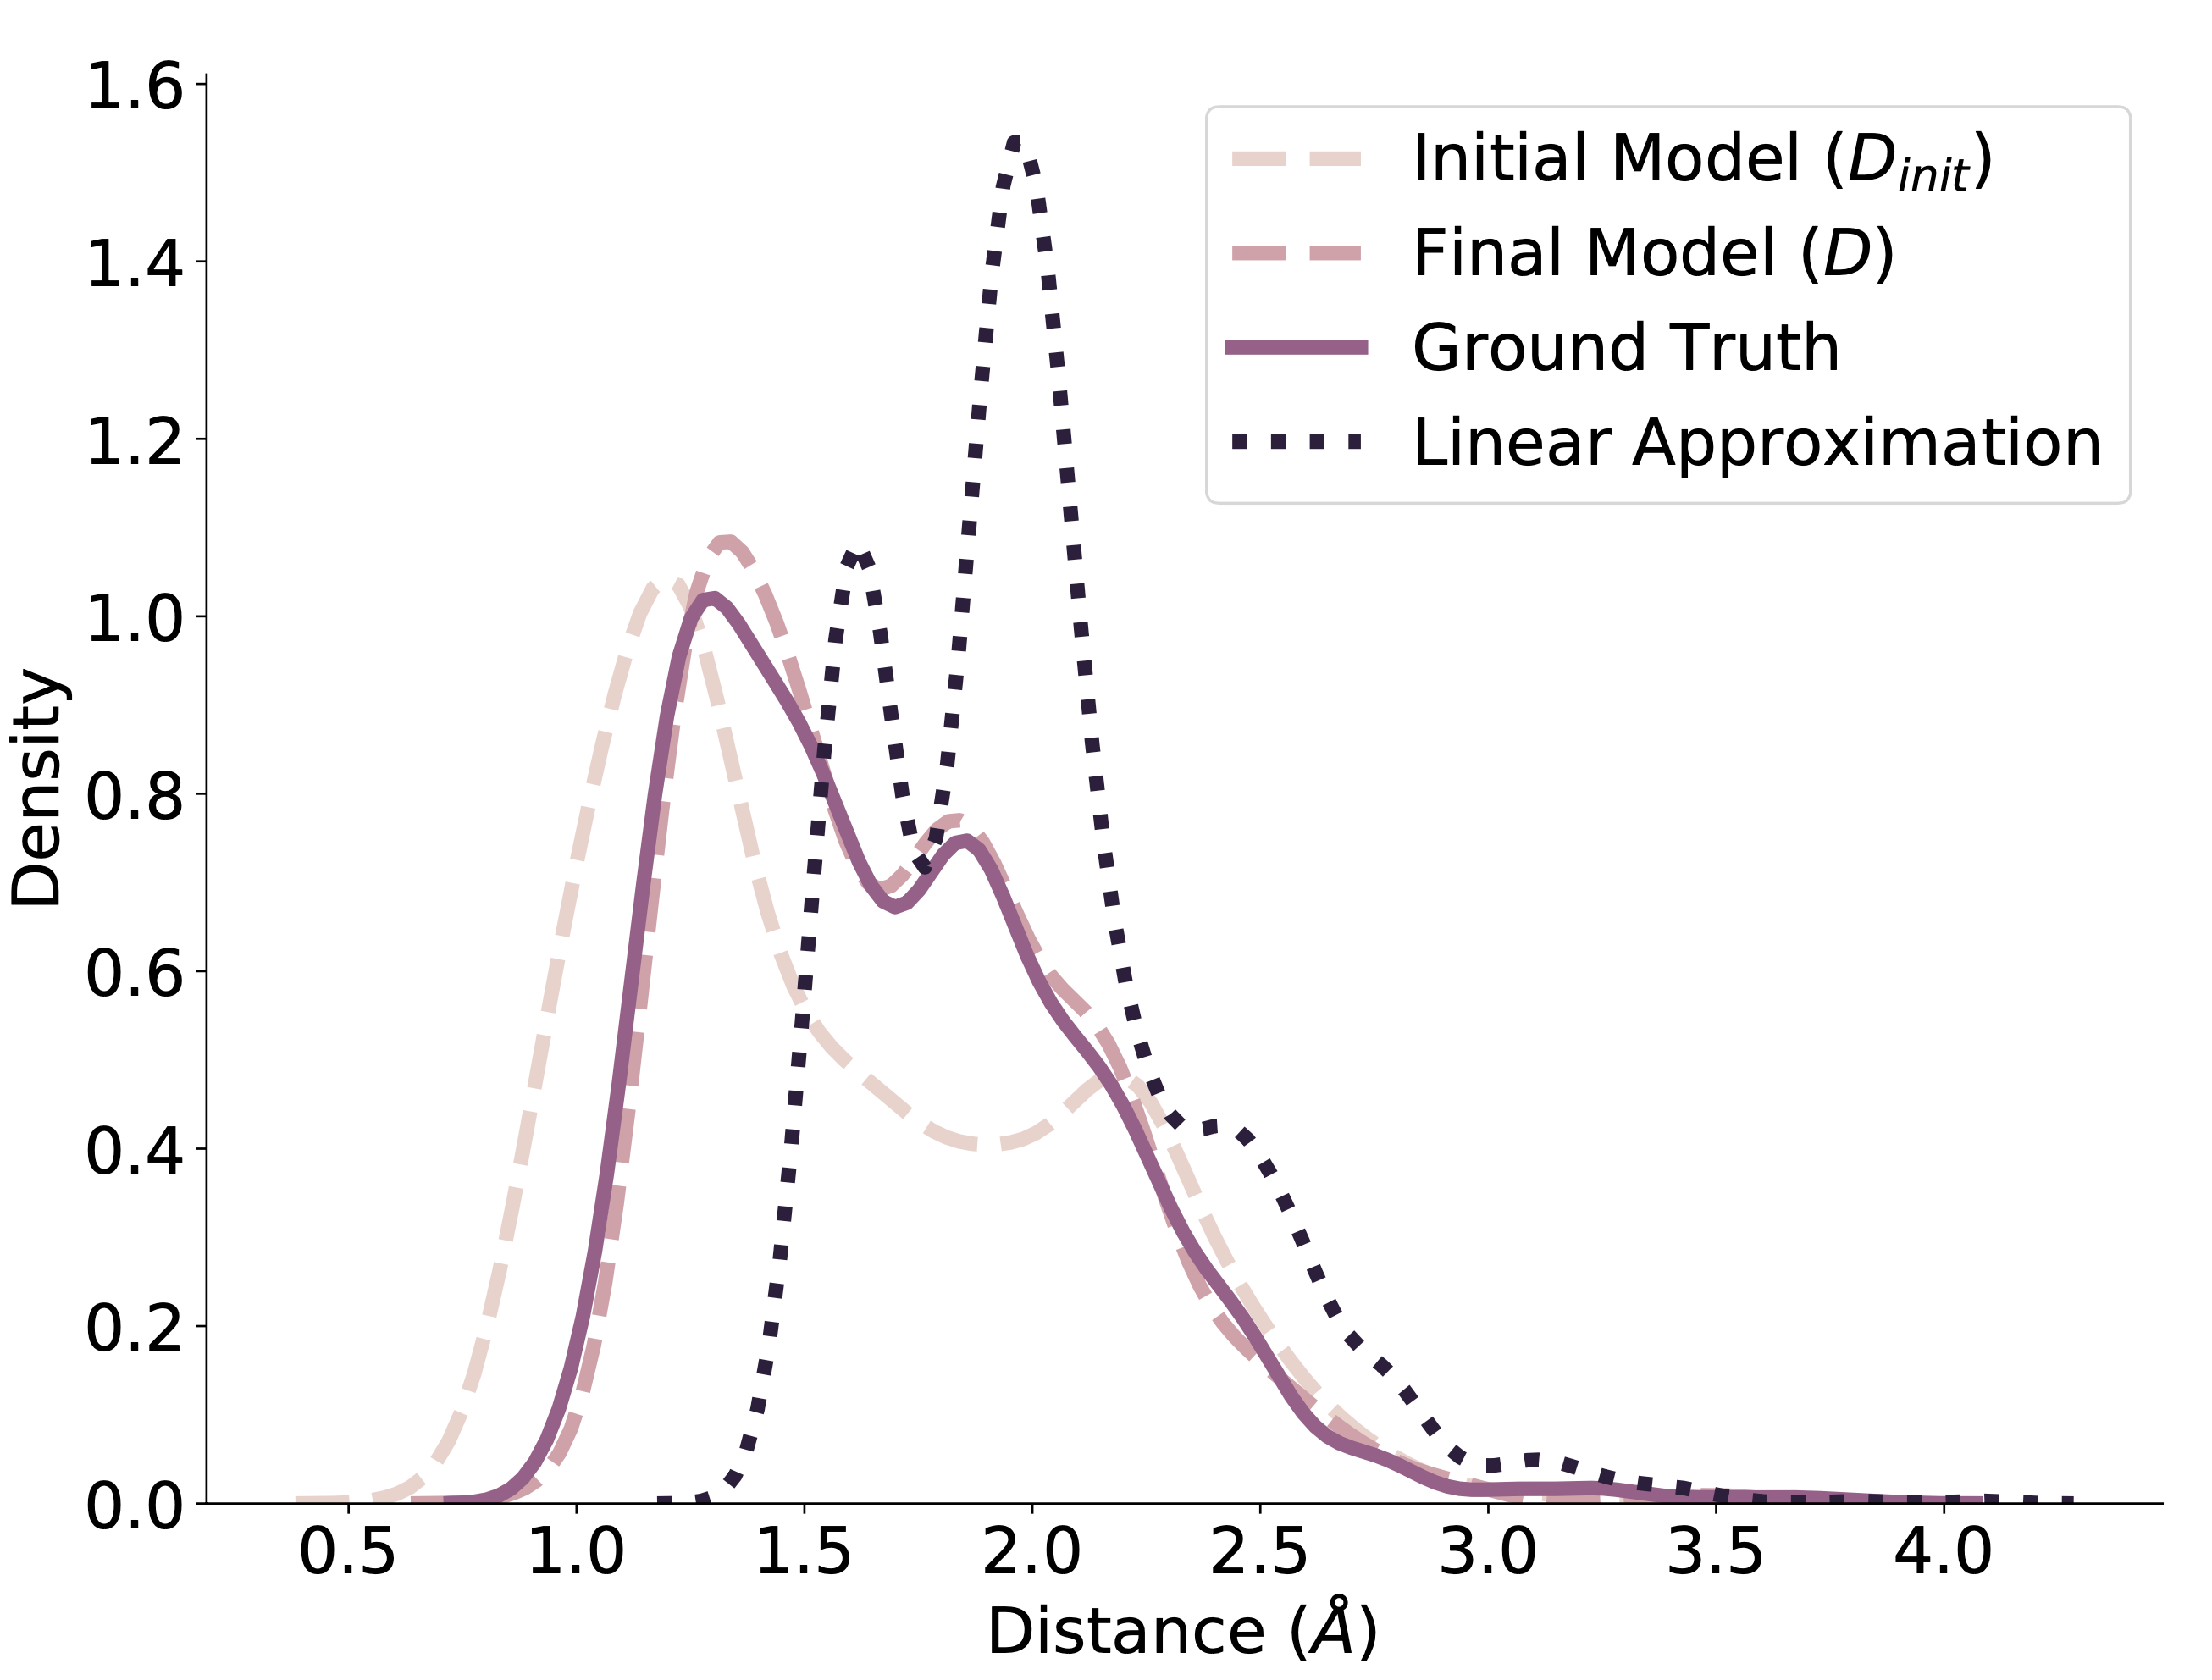
\includegraphics[width=0.5\textwidth]{ml-agreement}
    \caption{Initial model, final model, ground truth, and linear approximation of distance between atoms in the reacting core for the TS structures in the test set from \cite{pattanaik:2020}. }
    \label{fig:ml_agreement}
\end{figure}

TS Gen was tested on a set of 834 reactions and found 595 TS geometries that correctly matched ground truth reactants and products (71\%) with most failures coming from a number of uncommon reactions (i.e. reactions that do not match predefined reaction families in the Reaction Mechanism Generator \cite{gao:2016}).
Of their failed reactions, a majority of the failures stem from failed TS optimizations, mismatched calculated ground state structures, and failed ground state optimizations.
When comparing common reactions the authors had a success rate of 89\%.

Although the workflow can predict TS geometries with reasonable success, the authors comment that the current model is not adequate for multi-reactant reactions because of increased complexity when orienting multiple reactants together before generating a TS.

\subsection{RMSD-PP-TS (2020)}

The RMSD-PP-TS is a software that combines a meta-dynamics reaction path search with a series of local saddle point searches to find TS geometries for diverse elementary reactions \cite{rasmussen:2020}. 
An overview of the workflow is shown in \figref{fig:rmsd}.

\begin{figure}[htbp]
    \centering
    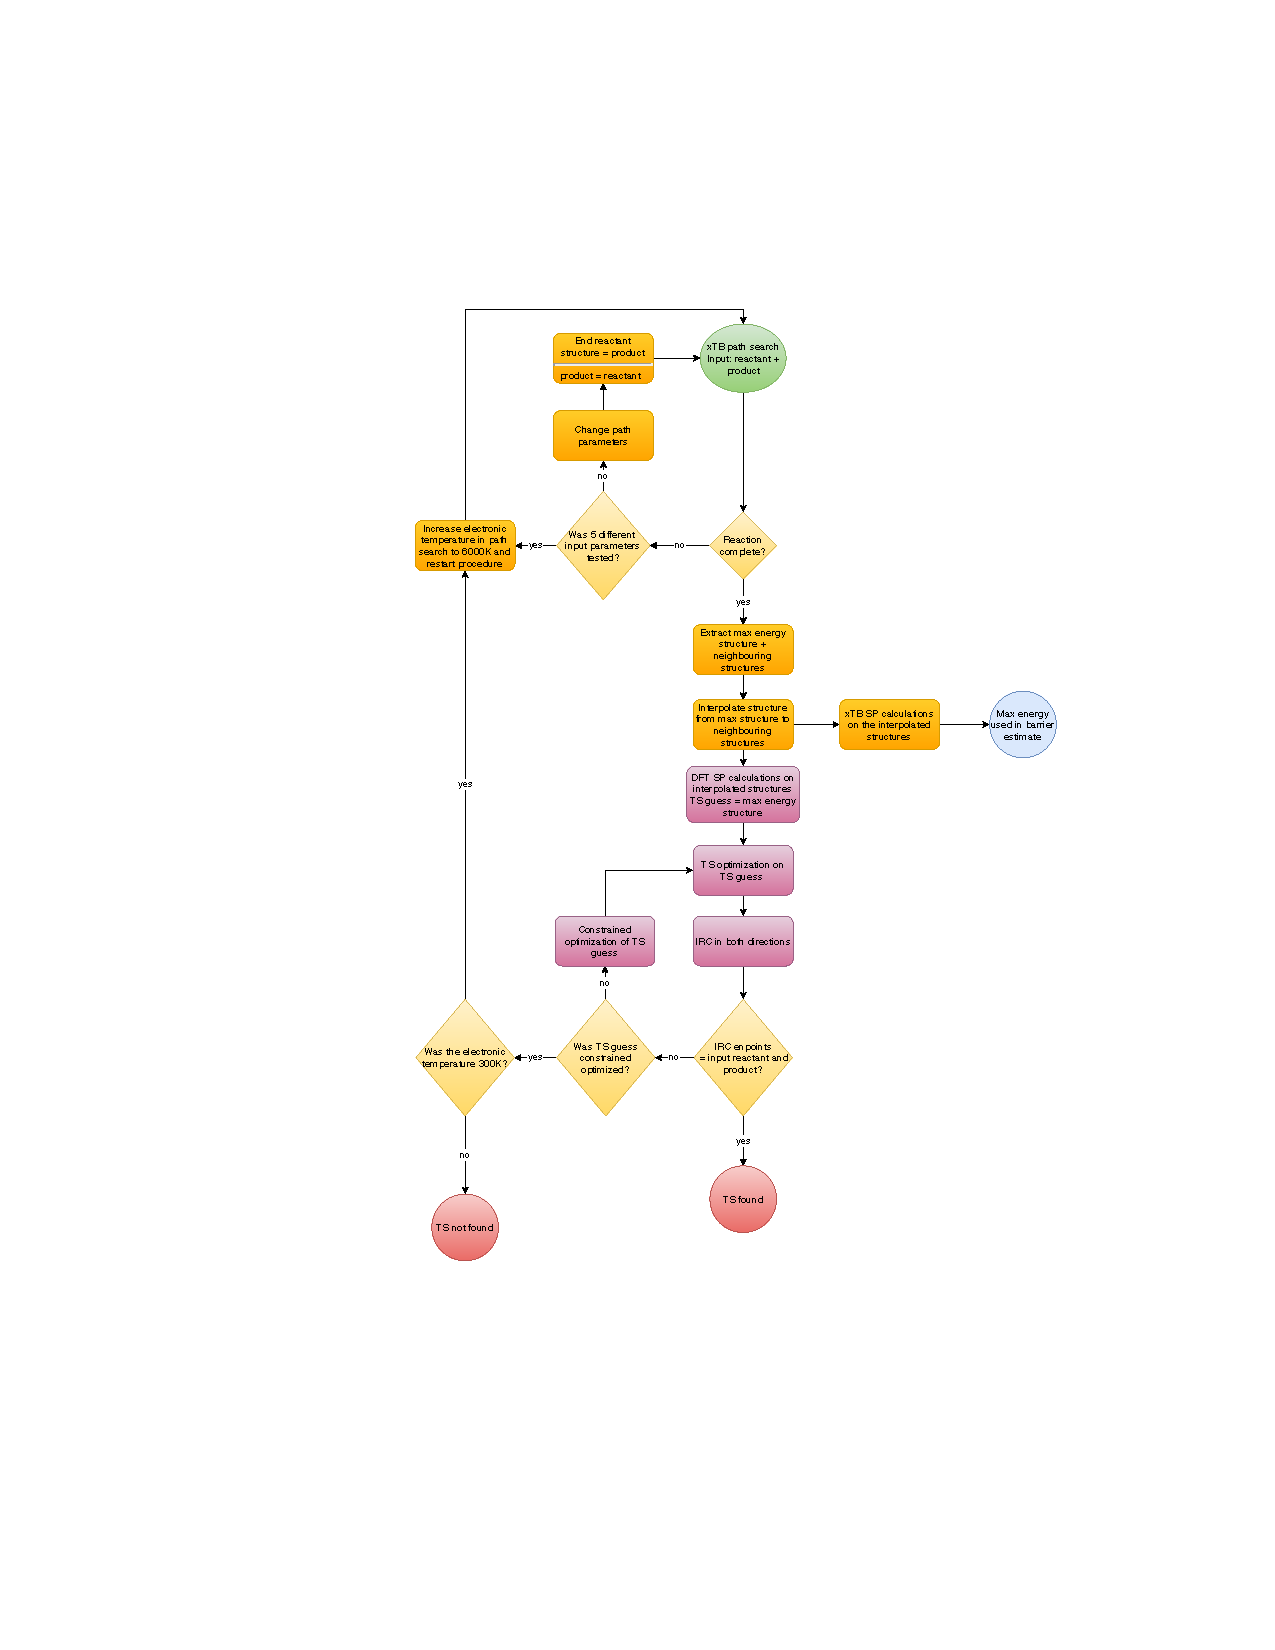
\includegraphics{rsmd}
    \caption{A workflow diagram describing the TS optimization method used in RMSD-PP-TS. Borrowed from \cite{rasmussen:2020}}
    \label{fig:rmsd}
\end{figure}

This software is based on the RMSD-PP method \cite{Grimme:2019} that performs reaction path analyses by applying artificial forces on subgroups of reactants and then uses a meta-dynamics simulation at a L1 level of theory to find product geometries.
These meta-dynamics simulations allow the complex to optimize to a constrained minima while preventing relaxation back to reactant geometries.

RMSD-PP-TS will use RMSD-PP to perform a reaction path analysis by first comparing the input reactant and product geometries.
A series of RMSD-PP path analyses are performed with a set of push and pull forces at a L1 level of theory at 300K.
A run is successful if the ending geometry from the RMDS-PP path analysis matches the input products.
If no path analyses are successful, the calculations are re-performed at a temperature of 6000K. 
The maximum energy value of the reaction path analysis will be used as the initial guess for the saddle point search. 

The saddle point search is performed at a L2 level of theory in Gaussian \cite{Gaussian:2009} and an IRC calculation is used for validation.
The Cartesian outputs of the IRC calculation are converted into adjacency matrices using RDKit \cite{RDKit:2018} and xyz2mol \cite{xyz2mol} and are compared to input geometries for reactants and products.
If the IRC endpoints do not match the inputs, the endpoints are further optimized at a L2 level of theory and compared again. 
%This is performed to insure that the IRC calculation results in energy minima.

If the IRC validation was unsuccessful, the TS guess undergoes a constrained to a minima optimization with reactive bonds frozen.
This new guess is then optimzied, IRC calculations are performed, it is validated again.
If a TS is still not found, the process is repeated using the RMSD-PP path analysis performed at 6000K.

The authors tested the workflow on a subset of reactions studied by Zimmerman \cite{Zimmerman:2013jctc,Zimmerman:2015jcc}.
This subset consists of 100 elementary reactions containing between 1 and 6 bond changes.
The authors' workflow was able to find 89 of 100 reactions successfully.
Although these results are promising, the authors note that RMSD-PP-TS will occasionally return false TSs when barrier heights are low and needs to be investigated.



\subsection{autodE (2020)}

One of the latest advances in automated TS searches is autodE \cite{young:2020} which calculates reaction profiles from a list of reactant and product SMILES strings using the workflow outlined in \figref{fig:autode}.
autodE interfaces with many electronic structure calculators (ORCA, Gaussian \cite{Gaussian:2009}, NWChem \cite{NWChem:2020}, MOPAC \cite{mopac:2016}, and XTB) \cite{xtb:2020} with either user-defined or suggested default methods.

\begin{figure}[htbp]
    \centering
    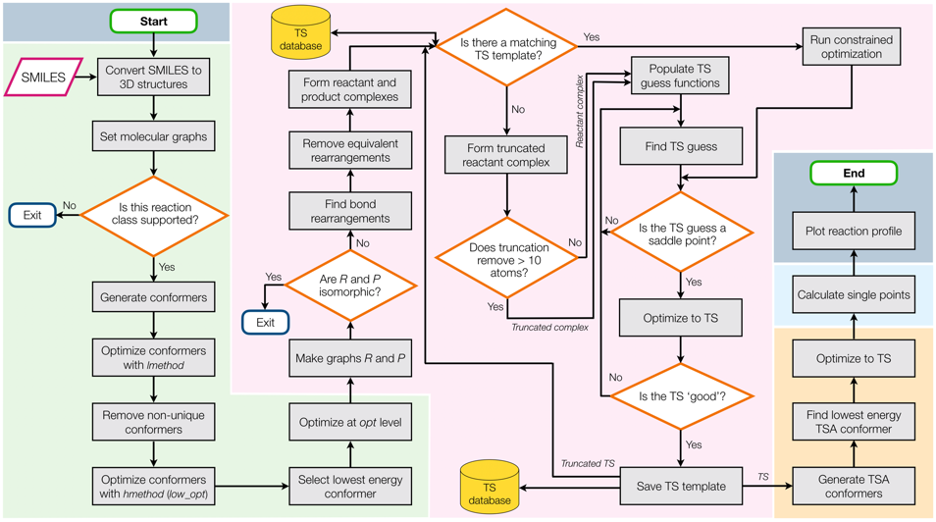
\includegraphics{autode}
    \caption{Workflow that is used by autodE to create reaction profiles from a set of reactant and product SMILES strings. The TS analogue (TSA) is the conformer analysis performed on the TS complex where active bonds are fixed. Taken from \cite{young:2020}.}
    \label{fig:autode}
\end{figure}

First, autodE will find a low energy conformer for reactants and products from SMILES strings by using the ETKDGv2 method implemented in RDKit \cite{RDKit:2018} for organic species.
For metallic complexes, the authors employ a custom conformer search method that adds each atom sequentially by placing it randomly in a 10 \AA~cubic box and minimizes a custom force field based on repulsion and bonding interactions.
Each conformer found is optimized with a lower level of theory to find an ensemble of conformers within an energy threshold (1 kJ/mol by default).
This ensemble is further optimized using a higher level of theory to find the lowest energy conformer. 

The set of reactants are merged to form a reactant graph where the atoms are vertices and the bonds are edges and the same is done for the products. 
Combinations of bonds in the reactant graph are iterated to perform a series of bond additions and bond breakages.
After each bond modification, the edited reactant graph is compared to the product graph to check for isomorphism using NetworkX \cite{networkx:2008}.

If the modified reactant and product graphs are isomorphic, a TS will either be generated via the ``truncation'' method or the ``template'' method. 
In the truncation method, autodE replaces \ce{C-X} bonds where the carbon atom is fully saturated with hydrogen atoms and it preforms a linear search between reactants and products to find the TS guess.
Once a guess has been found, the truncated bonds are replaced and the guess is optimized to a saddle point at a user defined higher level of theory (often L2).
In the template method, autodE will search its database of previously optimized TSs for a similar TS structure.
A database entry will be used if it has the same charge, multiplicity, solvent parameters, identical active bonds, and similar atoms (based on connectivity and atom type) near active bonds.
Non-matching bonds and atoms will be replaced in the template to match the TS of interest and will be optimized to a saddle point at a user defined higher level of theory.

The TS will be vetted to see if it is ``good'' (as shown in \figref{fig:autode}, meaning that the TS has exactly one imaginary frequency corresponding to a significant translation from the active bonds.
The forward and backward displacement will be used to run a quick reaction coordinate (QRC) calculation \cite{qrc:2003} to verify that the reactants and products from the TS correspond to the reactant and product graphs.

A TS analogous (TSA) conformer analysis will be performed on the vetted geometry to find lower energy conformer, if possible.
This mirrors the initial conformer analysis that is performed on stable species except distances between reacting atoms are constrained.
The conformers found are then optimized and lower energy conformers are vetted as ``good'' using above methods as well.
Finally, single point energies are calculated for each reactant, product, and TS, and a reaction profile is generated. 
van der Waals complexes can also be created along the reaction path at the users request.

The authors tested their workflow on approximately 100 diverse reactions and saw good success rates. 
The authors do note two immediate limitations of their methods: the need to define bonds and to check sterochemistry. 
The energy required to overcome a bond (whether covalent or non-covalent) does not necessarily correspond to the type of interaction. 
This tricky definition makes it hard to assign what a ``good'' TS is when active bonds may not lead to products or reactants. 
Additionally, the isomorphism check does not account for streochemistry.
Finally, autodE has issues when performing conformer analyses on anions which results in barrierless reactions. 





%%%%%%%%%%%%%%%%%%%%%%%%%%%%%%%%%%%%%%%%%%%%%%%%%%%%%%%%%%%%%%%%%%%%%%%%%%%%%%%%%%%%
%%%%%%%%%%%%%%%%%%%%%%%%%%%%%%%%%%%%%%%%%%%%%%%%%%%%%%%%%%%%%%%%%%%%%%%%%%%%%%%%%%%%
%%%%%%%%%%%%%%%%%%%%%%%%%%%%%%%%%%%%%%%%%%%%%%%%%%%%%%%%%%%%%%%%%%%%%%%%%%%%%%%%%%%%

\section{Discussion}
%

This review summarizes existing code bases that can perform automated TST calculations.
%But it is hard to definitively say one code is ``best'' because the definition of ``best'' is subjective and near impossible to define.
Though all of these code bases fall under the umbrella of automated TST calculations, each has features to tackle specific issues well.
FSM and molecularGSM provide unique double ended methods for finding saddle points; AutoMeKin utilizes a unique chemical dynamics simulations approach; AutoTST provides high throughput calculations that perform better than most rate estimations; AFIR applies artificial forces to find reaction pathways; AutoTS finds TS geometries for almost any reaction family; Genesys provides on the fly calculations with little user input; AARON handles reactions involving transition metals; EStokTP provides high fidelity rate constant expressions with less user input than traditional TS searches; and KinBot bridges the gap between mechanism generation and automated TST calculations. 
RMSD-PP-TS uniquely uses a reaction path analysis; TS-Gen implements a novel machine learning approach; and autodE can created detailed reaction profiles. 
This review identifies that many code bases contain the following:
\begin{enumerate}
    \item Input method,
    \item A method to generate a TS guess,
    \item A method to arrive at a TS geometry,
    \item Tools to validate a TS geometry,
    \item Conformer analysis,
    \item Consideration of hindered rotors,
    \item Addition of single-point energies,
    \item Calculation of symmetry number,
    \item and a way to determine kinetic parameters.
\end{enumerate}

Each of these categories plus a few more are summarized in \tabref{table:comparison}.

\begin{landscape}
\begin{singlespace}
\begin{footnotesize}
\tiny
\begin{longtable}{| p{0.5in} | p{0.25in} | p{0.6in} | p{1.0in} | p{0.6in}| p{0.45in}| p{0.5in }| p{0.3in}| p{0.2in}| p{0.5in}| p{0.45in}| p{0.5in}| p{0.5in} | p{0.45in} |}
\caption{\label{table:comparison}A table describing the reviewed codes that describes their differences.}\\
\hline
Software  &  
Year Published  & 
 Input  &  
 Generation of Guesses  &  
 Geometry Optimizations of TS Guess &  
 Conformer Analysis  & 
Validation  &  
\rotatebox[origin=c]{90}{Hindered} \rotatebox[origin=c]{90}{Rotors}  & 
\rotatebox[origin=c]{90}{Level of Theory for} \rotatebox[origin=c]{90}{Single Point Energies} &
Symmetry  &  
 Kinetics  &
Supported QM Software  &
Supported Atoms  &
 Open Source? Licensing?  \\ 
\hline
\hline
FSM & 2011 &  3D geometries of reactants and products  & String method connecting reactants and products, string is a straight line recalculated using newest points & Native surface walking algorithm at L2 & No &  IRC Calculation  & No & L2 & No & No & Q-Chem & All atom types &  No, proprietary license  \\ 
\hline
molecular GSM & 2011 &  3D geometries of reactants and products for double ended method, reactants for single ended method & String method connecting reactants and products, string is a fitted curve recalculated using newest points & Native surface walking algorithm at L2 & No &  IRC Calculation  & No & L2 & No & No & Gaussian, MolPro, Orca, Q-Chem & All atom types &  Yes, MIT license  \\ 
\hline
AutoMeKin & 2014 &  3D geometries of reactants and products  & Chemical dynamics calculation performed to observe breaking / forming of bonds over a time scale, the point of change geometry is used as the starting guess & L1 optimization followed by an L1 validation, L2 reoptimization & No &  IRC Calculation  & No & L2 & No & No & MOPAC, Gaussian & All atom types &  Yes, MIT license  \\ 
\hline
AutoTST  & 2016 &  RMG reaction, reaction family  &  Identifies key distances based on functional groups in reaction center, embeds at L0.  &  Series of partial optimizations at L2  &  No  &  IRC Calculation  &  No  & L2 &  Yes, SYMMETRY package in RMG  &  Yes, Arkane  &  Gaussian  &  H, C, O. Partial support for Cl, N, S, Si  &  Yes, MIT license  \\ 
\hline
AFIR & 2016 &  3D geometries of reactants and products  & Reacting atoms are pushed together or pulled apart, the energy maximum is used as the starting guess & L2 optimization of energy maximum TS guesses & No &  IRC Calculation  & No & L2 & No & No & Gaussian & All atom types &  No, proprietary license  \\ 
\hline
AutoTS   & 2017 &  3D geometries of reactants and products  &  IDs active bonds through systematic deletion, Linear regression along reaction coordinates to find energy maximum at L2. Templates previous run reaction to reaction of interest.  &  QST search using reactants, products, and TS guess at L2  &  No  &  Vetting and Connecting  &  No  & L2 &  No  &  No  &  Jaguar  &  All atom types  &  No, proprietary license  \\ 
\hline
Genesys  & 2018 &  Guess of reaction center coordinates, reaction family  &  Uses key distances to embed with L0  &  Low level optimization and Conformer analysis at L1, Final optimization at L2  &  Yes, systematic  &  Normal mode analysis  &  Yes, 1D  & L3  &  Unspecified  &  Yes, by hand  &  Gaussian &  H, C, O, S  &  No, not distributed  \\ 
\hline
AARON    & 2018 &  Reaction template, labeled atoms  &  Template previous run reaction to reaction of interest  &  Partial optimizations at L2  &  Yes, rule based  &  ``Step Vetting'' Validation  &  No  & L2 &  No  &  No  &  Gaussian  &  All atom types  &  Yes, GPL-3.0 license  \\ 
\hline
EStokTP  & 2018 &  Guesses of reaction center coordinates, reaction family  &  Uses provided internal coordinates to construct 3D geometry  &  Conformer search at L2, series of partial optimizations at L2 theory  &  Yes, stochastic  &  IRC Calculation  & Yes, 1D, 2D, 3D  & L3  &  Yes, MESS package  &  Yes, AITSTME  &  Gaussian, MolPro  &  H, C, O, S, N  &  Yes, GPL-3.0 license   \\ 
\hline
KinBot   & 2019 &  SMILES or 3D coordinates of reactant, reaction families of interest  &  Indirect or direct setting of reaction center, relaxation of reaction shell. Scan along active bonds.   &  L0 search for conformer analysis, L2 search for final optimization.  &  Yes, systematic or random  &  IRC Calculation  &  Yes, 1D  & L2 &  Yes, graph based approach  &  Yes, MESS or MESMER  &  Gaussian  &  H, C, O, S  &  Yes, BSD 3-Clause license  \\ 
\hline
RMSD-PP-TS & 2020 & 3D coordinates of reactants and products & Use the energy maximum complex of a reaction path analysis. & Single optimization to a saddle point at L2 & No & IRC Calculation & No & L2 & No & No & Gaussian & Elements up to Z=86 & Yes, MIT license 
\\
\hline
TS Gen & 2020 & Unknown & Graph Neural Network & Single optimization to a saddle point at L2 & No & IRC Calculation & No & L2 & No & No & Gaussian & H, C, N, O & Yes, MIT license 
\\
\hline 
autodE & 2020 & SMILES of reactants and products & Truncating or Tempting methods with linear interpolation at user defined lower level & Single optimization to a saddle point as a user defined higher level & Yes, ETKDGv2 for organics and stochastics method for metal containing complexes & QRC calculation & No & L2 & No & No & ORCA, Gaussian, NWChem, MOPAC, XTB & Elements up to Z=86 & Yes, MIT license \\
\hline

\end{longtable}
\end{footnotesize}
\end{singlespace}
\end{landscape}

%In addition, each of these code bases lies somewhere on the plot of fidelity vs throughput. 
%We suggest a qualitative comparison of fidelity vs throughput for previously discussed code bases, rate rule estimations, and parameters determined via experimentation in \figref{fig:autokin_comparison}.
Though each of these code bases are effective, there is currently no tool that attains both the high throughput \textit{and} high fidelity required to calculate kinetic rates for entire reaction mechanisms.
The end goal of automated kinetics should strive for open-source codes that allow users to perform high fidelity TST calculations on reactions involving any atom type and for all reaction families (homo- and heterogeneous).
This software should: require simple inputs to create an educated guess of the TS geometry, perform a through conformational analysis and hindered rotor scans on all reactants, products, and TS geometries, calculate zero point energies, calculate symmetry numbers of complexes accurately, and estimate kinetic parameters while being able to work on a variety of reaction types, atom types, quantum software packages, and high performance computing environments.

AutoTST, AutoTS, AARON, KinBot, TS-Gen, and autodE allow libraries of previous results to generate TS guesses but FSM, molecularGSM, AutoMeKin, AutoTS, AFIR, RMSD-PP-TS, and autodE are able to provide these guesses without training data.
Being able to generate TSs with and without training data is highly sought after and should be included in future developments of softwares.
In addition, generalizability is desired.
FSM, molecularGSM, AutoMeKin, AutoTS, AFIR, AARON, RMSD-PP-TS, and autodE support many atom types and AutoTS can perform calculations on almost any reaction family, both of these features should be included in future software.
A detailed conformational analysis is of great importance and the stochastic and systematic methods that exist in AARON, KinBot, Genesys, EStokTP, and autodE allow for effective exploration of conformational space.
Hindered rotor scans and zero point energy calculations in KinBot, Genesys, and EStokTP help to more accurately estimate the kinetics of a reaction.
Finally, the determination of symmetry numbers and coupling to a statistical mechanics or master equation solver is necessary to obtain kinetics and is currently present in AutoTST, Genesys, KinBot and EStokTP.

The presence of many code bases is advantageous to perpetuate research through competition, but it can also be inefficient.
A collaborative effort should be made, when possible, to allow codes and their developers to interact and communicate with one another to further develop the field of automated TST.



\section{Acknowledgements}

This material is based upon work supported by the National Science Foundation under Grant No. 1605568.
The authors were partially supported by the U.S. Department of Energy, Office of Science, Basic Energy Sciences, under Award \#0000232253, as part of the Computational Chemical Sciences Program.


\rhw{Remove the arXiv preprint links that are incorrect and the redundant URLs}

\bibliography{refs.bib}
\bibliographystyle{elsarticle-num}



\end{document}
